\documentclass[10pt]{beamer}
\usepackage{amsmath}
\usepackage{amssymb}
%\usepackage{dsfont}
\usepackage{accents}
\usepackage{hyphenat}
\usepackage{multirow}
\usepackage{animate}
\usetheme[progressbar=frametitle]{metropolis}
\setbeamercolor{background canvas}{bg=white}
% \usetheme{focus}
\usepackage{appendixnumberbeamer}
\usefonttheme[onlymath]{serif}
\usepackage{booktabs}
\usepackage[scale=2]{ccicons}

\usepackage{pgfplots}
\usepgfplotslibrary{dateplot}

\usepackage{xspace}
\newcommand{\themename}{\textbf{\textsc{metropolis}}\xspace}
\usetikzlibrary{snakes,arrows,mindmap,trees,backgrounds,shapes.geometric,calc}
\tikzset{graphics/.style={inner sep=0,outer sep=0}}
\tikzset{scaleall/.style={scale=#1, transform shape}}
\usepgflibrary{arrows}


\newlength{\bbw}
\newlength{\bbh}
\newcommand{\pcuad}[3][]{
  % First arguments is an optional prefix for the coordinate names

  \setlength{\bbw}{#2}
  \setlength{\bbh}{#3}
  \useasboundingbox(0,0) rectangle (\bbw,\bbh);

  \path(.5\bbw,.5\bbh) coordinate(#1cp);
  \path(\bbw,0)        coordinate(#1se);
  \path(0,0)           coordinate(#1sw);
  \path(0,\bbh)        coordinate(#1nw);
  \path(\bbw,\bbh)     coordinate(#1ne);
 
  
  \path(\bbw,.5\bbh) coordinate(#1ep);
  \path(.5\bbw,0)    coordinate(#1sp);
  \path(.5\bbw,\bbh) coordinate(#1np);
  \path(0,.5\bbh)    coordinate(#1wp);
       
  \path(.75\bbw,.5\bbh) coordinate(#1hr);
  \path(.25\bbw,.5\bbh) coordinate(#1hl);
  \path(.5\bbw,.25\bbh) coordinate(#1vl);
  \path(.5\bbw,.75\bbh) coordinate(#1vu);

  \path(.75\bbw,.75\bbh) coordinate(#1c1);
  \path(.25\bbw,.75\bbh) coordinate(#1c2);
  \path(.25\bbw,.25\bbh) coordinate(#1c3);
  \path(.75\bbw,.25\bbh) coordinate(#1c4);


%  +-----------------------------------------------+
%  |nw                    np                     ne|
%  |                                               |
%  |                                               |
%  |          c2          vu          c1           |
%  |                                               |
%  |                                               |
%  |wp        hl          cp          hr         ep|
%  |                                               |
%  |                                               |
%  |          c3          vl          c4           |
%  |                                               |
%  |                                               |
%  |sw                    sp                     se|
%  +-----------------------------------------------+
}
 
        
\newcommand{\showcuad}[1][]{

   \draw[help lines,xstep=.5,ystep=.5,gray!10] (#1sw) grid (#1ne);
   \draw[help lines,xstep=1,ystep=1,gray]      (#1sw) grid (#1ne);
   %\draw[help lines,xstep=.25,ystep=.25,gray!20] (sw) grid (ne);
   % \draw[help lines,xstep=1,ystep=1,gray] (sw) grid (ne);
   % \foreach \x in {-20,-14.5,...,20} {
   %     \node [anchor=north, gray,yshift=30] at (\x,0) {\tiny \bf \x};
   %     \node [anchor=east,gray,xshift=30] at (0,\x) {\tiny \bf  \x};
   % }
               
    \fill(#1se) circle(.1) node[anchor=south east]{#1se};
    \fill(#1sw) circle(.1) node[anchor=south west]{#1sw};
    \fill(#1ne) circle(.1) node[anchor=north east]{#1ne};
    \fill(#1nw) circle(.1) node[anchor=north west]{#1nw};
                  
    \fill(#1hr) circle(.1) node[above]{#1hr};
    \fill(#1hl) circle(.1) node[above]{#1hl};
    \fill(#1vu) circle(.1) node[above]{#1vu};
    \fill(#1vl) circle(.1) node[above]{#1vl};
                  
    \fill(#1sp) circle(.1) node[anchor=south]{#1sp};
    \fill(#1wp) circle(.1) node[anchor=west] {#1wp};
    \fill(#1np) circle(.1) node[anchor=north]{#1np};
    \fill(#1ep) circle(.1) node[anchor=east] {#1ep};

    \fill(#1cp) circle(.1) node[above]{#1cp};
    \fill(#1c1) circle(.1) node[above]{#1c1};
    \fill(#1c2) circle(.1) node[above]{#1c2};
    \fill(#1c3) circle(.1) node[above]{#1c3}; 
    \fill(#1c4) circle(.1) node[above]{#1c4};

    %\fill[red](cp|-c1) circle(.1) node[anchor=north]{cp|-c1};

}

\newcommand{\ds}{\displaystyle}
\newcommand{\dsum}{\displaystyle \sum}
\newcommand{\uu}[1]{{\boldsymbol #1}}
\newcommand{\ud}{\,\mathrm{d}}
\def\ttau{\uu{\tau}}
\def\bb{\uu{b}}
\def\nb{\uu{n}}
\def\pb{\uu{p}}
\def\wb{\uu{w}}
\def\xb{\uu{x}}
\def\ab{\uu{a}}
\def\mb{\uu{m}}
\def\yb{\uu{y}}
\def\vb{\uu{v}}
\def\fb{\uu{f}}
\def\zb{\uu{z}}
\def\Xb{\uu{X}}
\def\etab{\uu{\eta}}
\def\thetab{\uu{\theta}}
\def\lambdab{\uu{\lambda}}
\def\gammab{\uu{\gamma}}
\def\taub{\uu{\tau}}
\def\varphib{\uu{\varphi}}
\def\Ab{\uu{A}}
\def\Bb{\uu{B}}
\def\Gb{\uu{G}}
\def\Fb{\uu{F}}
\def\Jb{\uu{J}}
\def\Rb{\uu{R}}
\def\Tb{\uu{T}}
\def\rb{\uu{r}}
\def\ab{\uu{a}}
\newcommand{\molar}[1]{\underaccent{\bar}{#1}}
\def\um{\molar{U}}
\def\hm{\molar{H}}
\def\sm{\molar{S}}
\def\am{\molar{A}}
\def\gm{\molar{G}}
\def\hh{\hat{H}}
\def\sh{\hat{S}}
\def\vm{\molar{V}}
\def\cp{C_{\rm P}}
\def\cv{C_{\rm V}}
\def\cps{C_{\rm P}^*}
\def\cvs{C_{\rm V}^*}
\def\wsd{\dot{W}_s}
\def\md{\dot{M}}\newcommand{\pd}[2]{\left(\frac{\partial {#1}}{\partial 
{#2}}\right)}
\newcommand{\tpd}[3]{\left(\frac{\partial {#1}}{\partial {#2}}\right)_{#3}}
\newcommand{\tpdn}[4]{\left(\frac{\partial^{#4} {#1}}{\partial 
{#2}^{#4}}\right)_{#3}}



\title{Recent simulation methods for resolving molecular thermodynamics}
\date{May 20, 2021}
\author{Cameron F. Abrams}
\institute{Drexel University, Department of Chemical and Biological Engineering}
\titlegraphic{\hfill
\includegraphics[height=0.75cm]{drexel-horz-blue.png}}

\begin{document}

\maketitle

\section{Introduction and Motivation:  Making MD Do More}

\tikzstyle{startstop} = [rectangle, rounded corners, minimum width=1cm, minimum height=0.5cm,text centered, draw=black, fill=red!30]
\tikzstyle{io} = [trapezium, trapezium left angle=70, trapezium right angle=110, minimum width=1cm, minimum height=0.5cm, text centered, draw=black, fill=blue!30]
\tikzstyle{process} = [rectangle, minimum width=1cm, minimum height=1cm, text centered, draw=black, fill=orange!30]
\tikzstyle{decision} = [diamond, minimum width=1cm, minimum height=1cm, text centered, draw=black, fill=green!30]
\tikzstyle{myarrow} = [thick,->,>=stealth]
\begin{frame}[fragile]{Molecular Dynamics (MD)}
\begin{tikzpicture}[scaleall=1.0,node distance=2cm]
\node (start) [startstop] {Start};
\node (init) [io,right of=start,xshift=1cm,text width=2cm] {Initial atomic positions and velocities};
\node (force) [process,right of=init,xshift=1cm] {Get forces};
\node (integrate) [process,below of=force] {Update positions and velocities};
\node (check) [decision,below of=integrate] {Done?};
\node (continue) [process,right of=check,xshift=1cm] {\begin{tabular}{c} Update time \\ by 10$^{-15}$ s \end{tabular}};
\node (terminate) [process,left of=check,xshift=-1cm] {Save data};
\node (stop) [startstop,left of=terminate] {Stop};
\draw [myarrow] (start) -- (init);
\draw [myarrow] (init) -- (force);
\draw [myarrow] (force) -- (integrate);
\draw [myarrow] (integrate) -- (check);
\draw [myarrow] (check) -- node[anchor=south] {no} (continue);
\draw [myarrow] (continue) |- (force);
\draw [myarrow] (check) -- node[anchor=south] {yes} (terminate);
\draw [myarrow] (terminate) -- (stop);
\end{tikzpicture}
\end{frame}


\tikzstyle{label} = [rectangle, rounded corners, minimum width=1cm, minimum height=0.5cm,text centered, draw=black, fill=red!30]
\begin{frame}{Macrostates and Microstates}
\begin{tikzpicture}[scaleall=1.0,node distance=3cm]]
\node (pic) [] {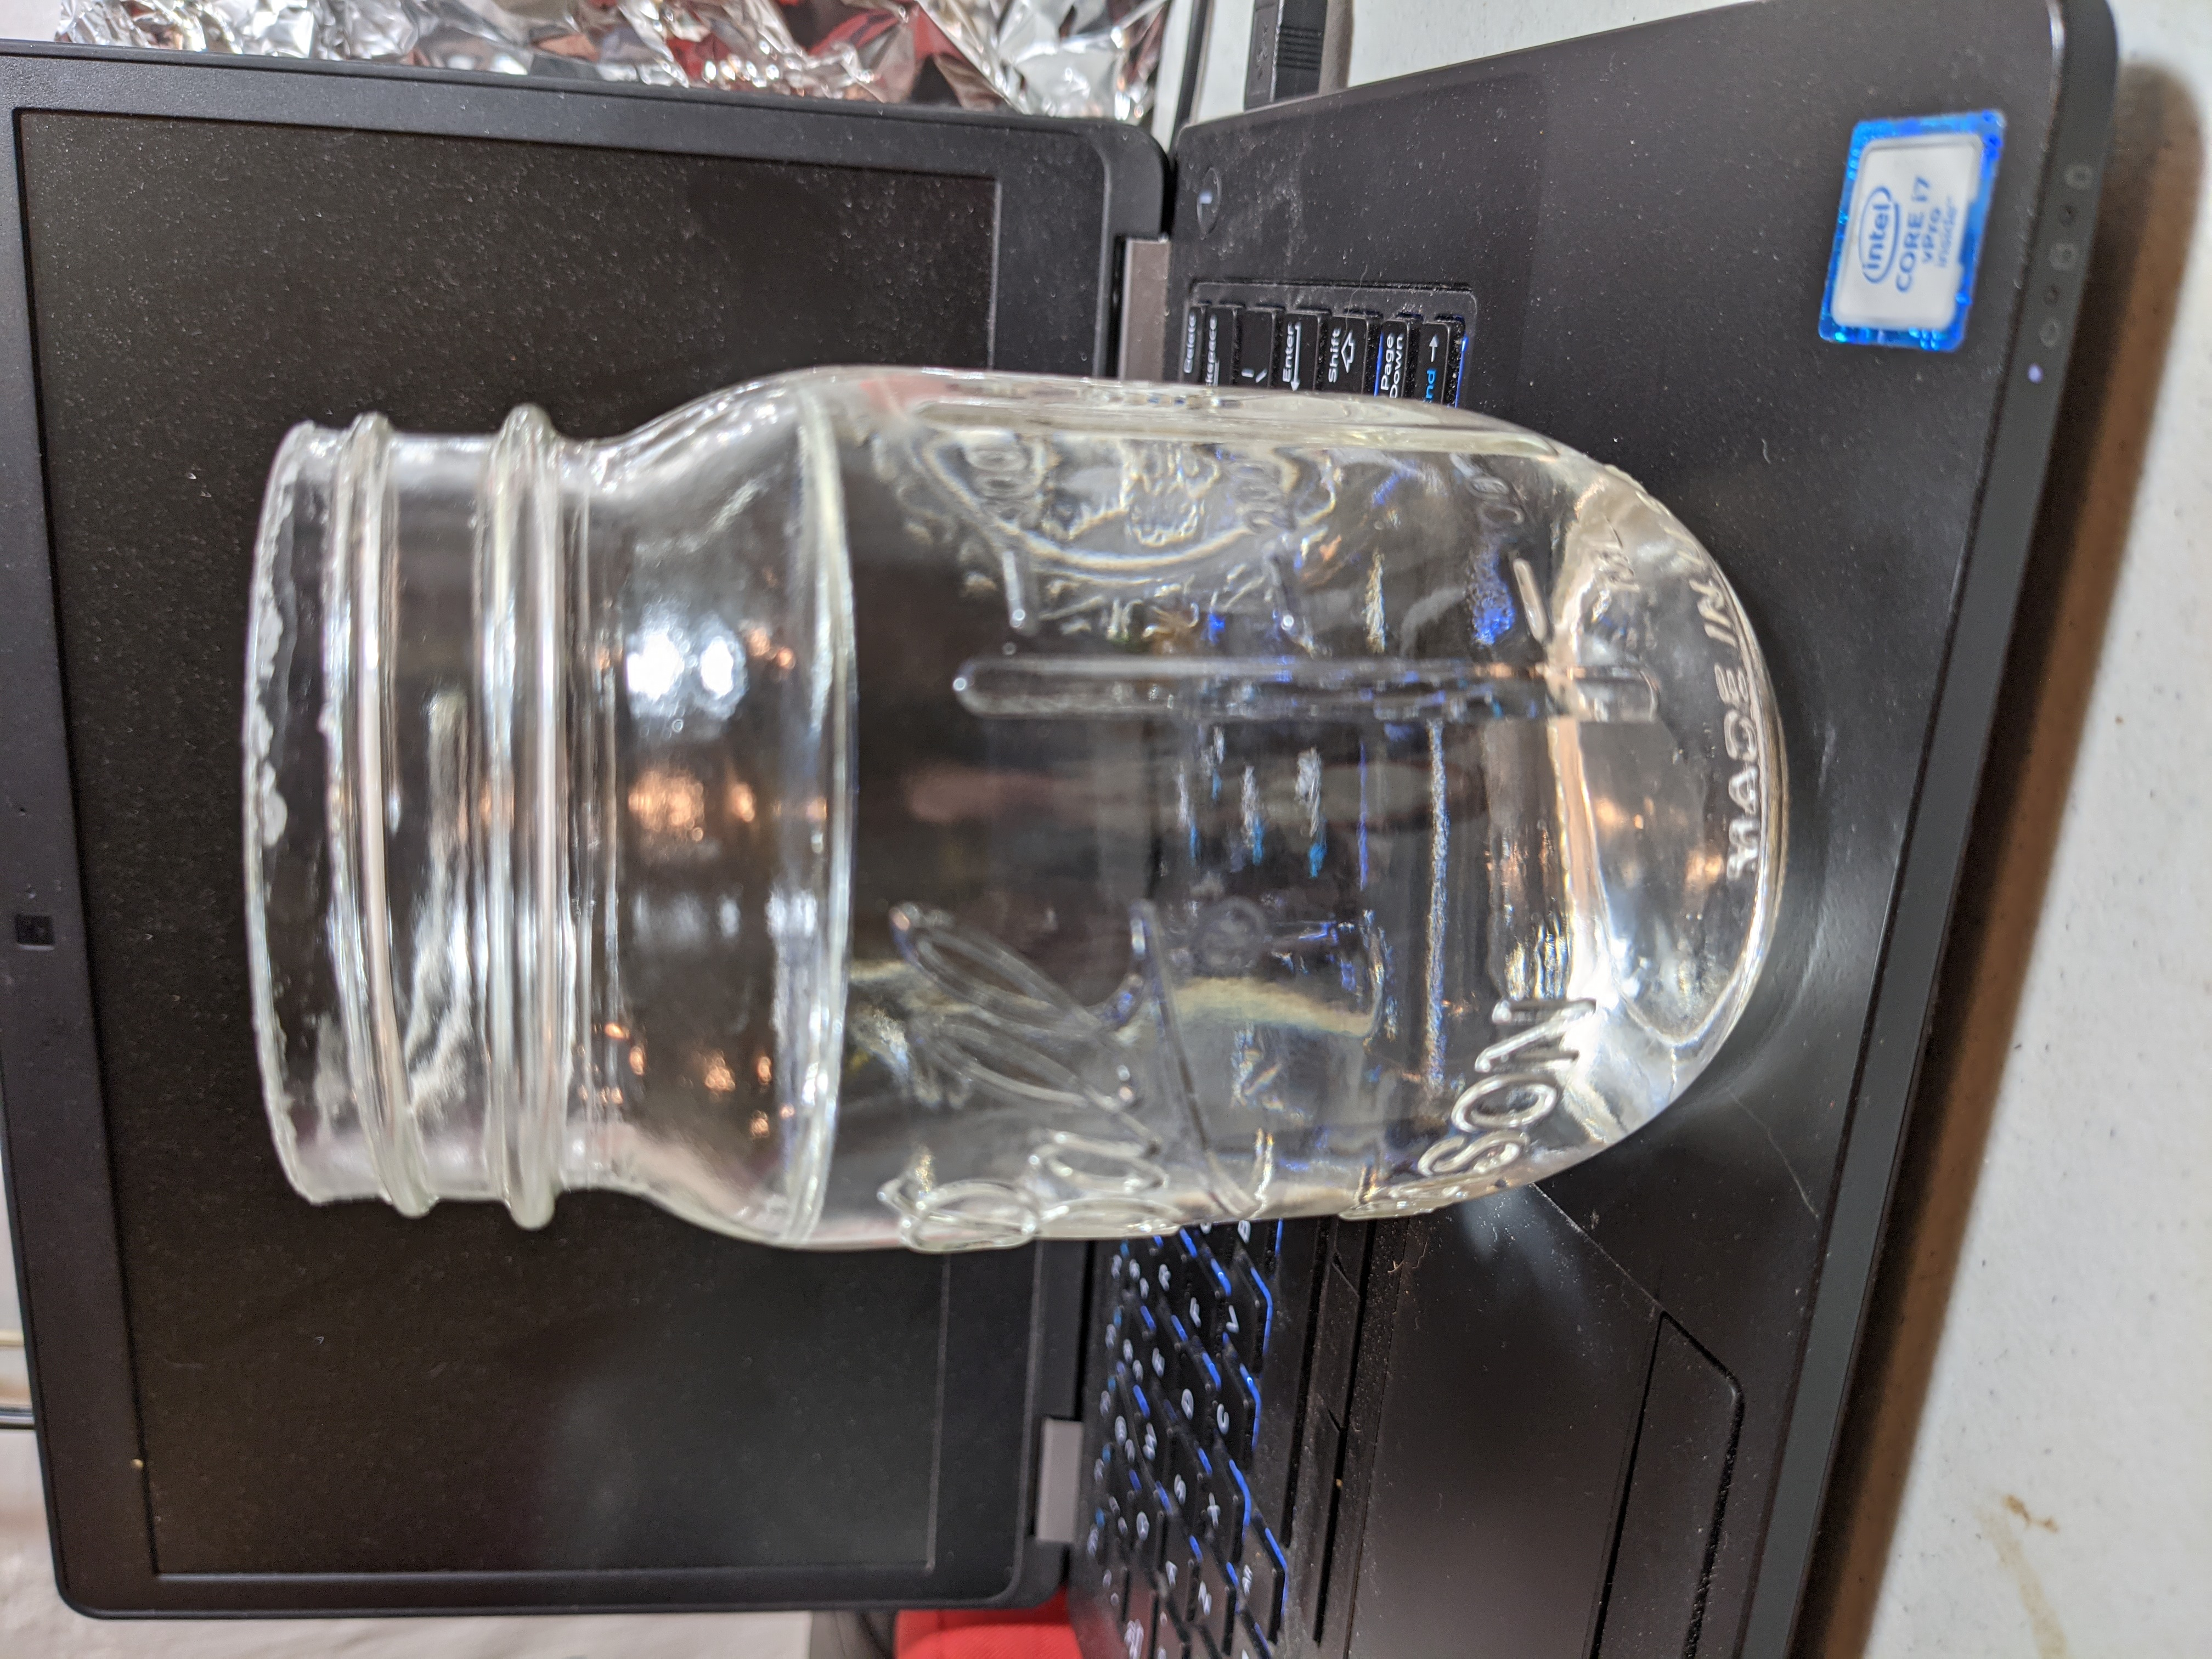
\includegraphics[angle=270,width=0.4\textwidth]{water-pic.jpg}};
\node (label1) [label,below of=pic,yshift=-1cm] {Macrostate}; 
\node (graphic1) [right of=pic,xshift=3cm,yshift=-0.1cm] {
        \animategraphics[loop,controls,width=0.5\textwidth]{10}{../movie-water-md/water.000}{00}{90}
    };
\node (label2) [label,below of=graphic1,yshift=-0.9cm] {Microstates (MD)}; 
\end{tikzpicture}
\end{frame}

\begin{frame}[fragile]{Lengthening the Reach of Molecular Dynamics Simulations}
%\vspace{5mm}
%\hspace{-5mm}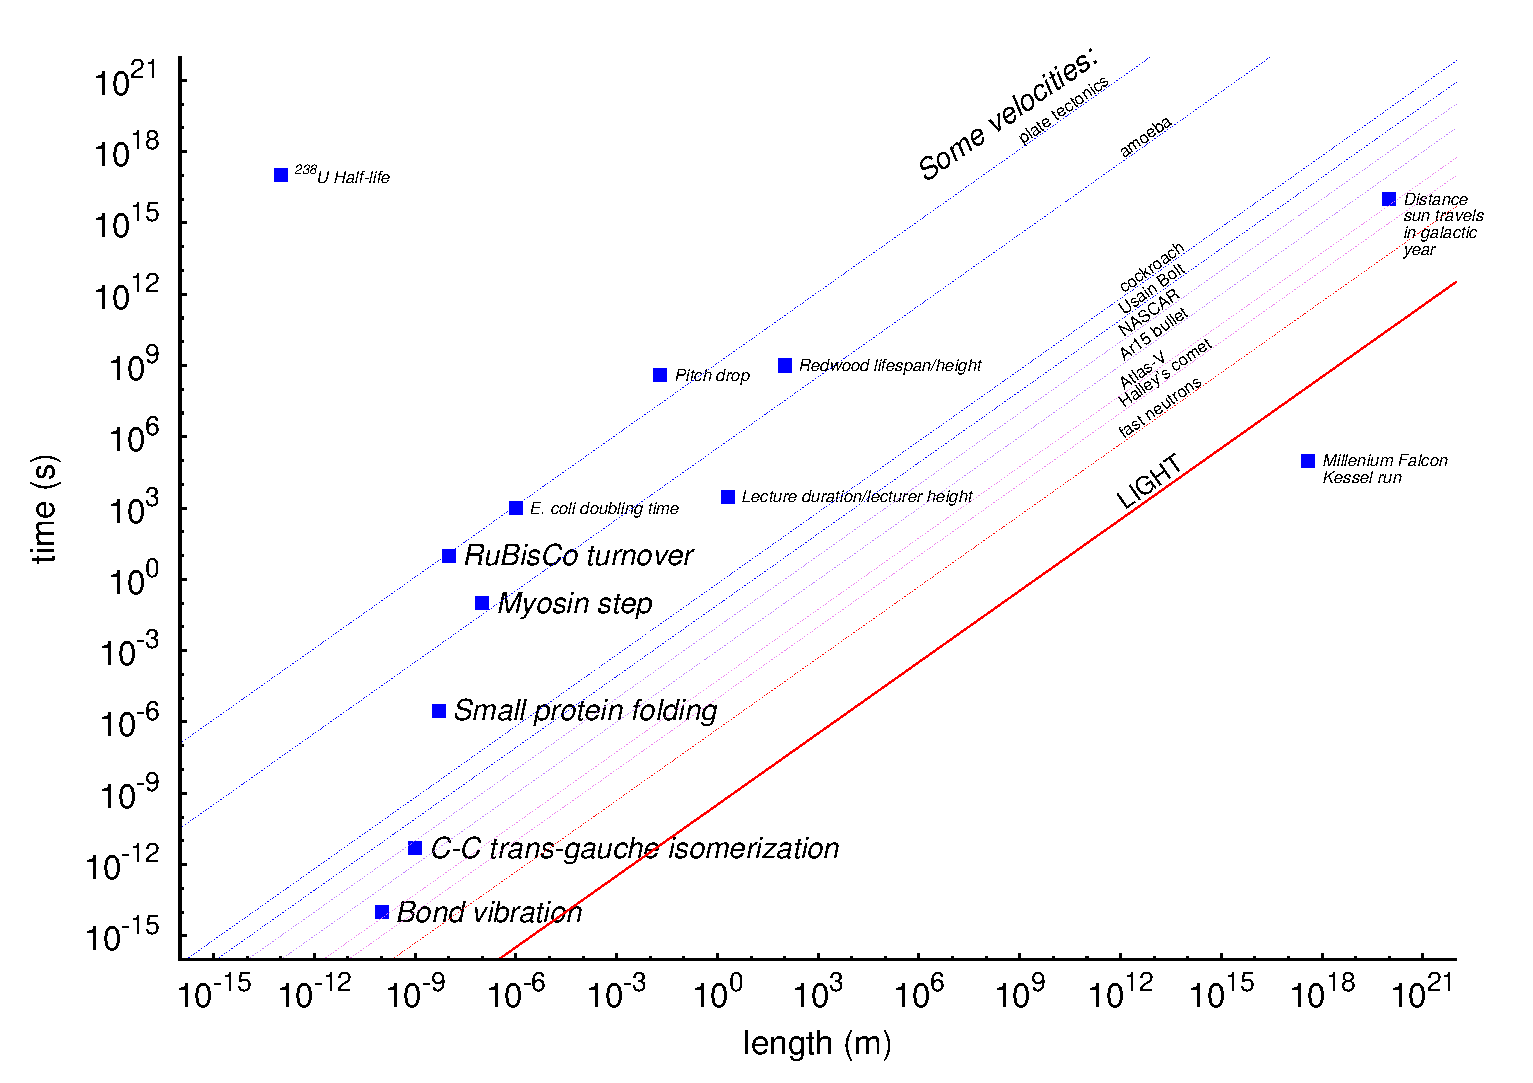
\includegraphics[width=\textwidth]{time_vs_length.eps}
\begin{tikzpicture}[scale=1.5]
\node[anchor=south west,inner sep=0] (image) at (0,0) 
{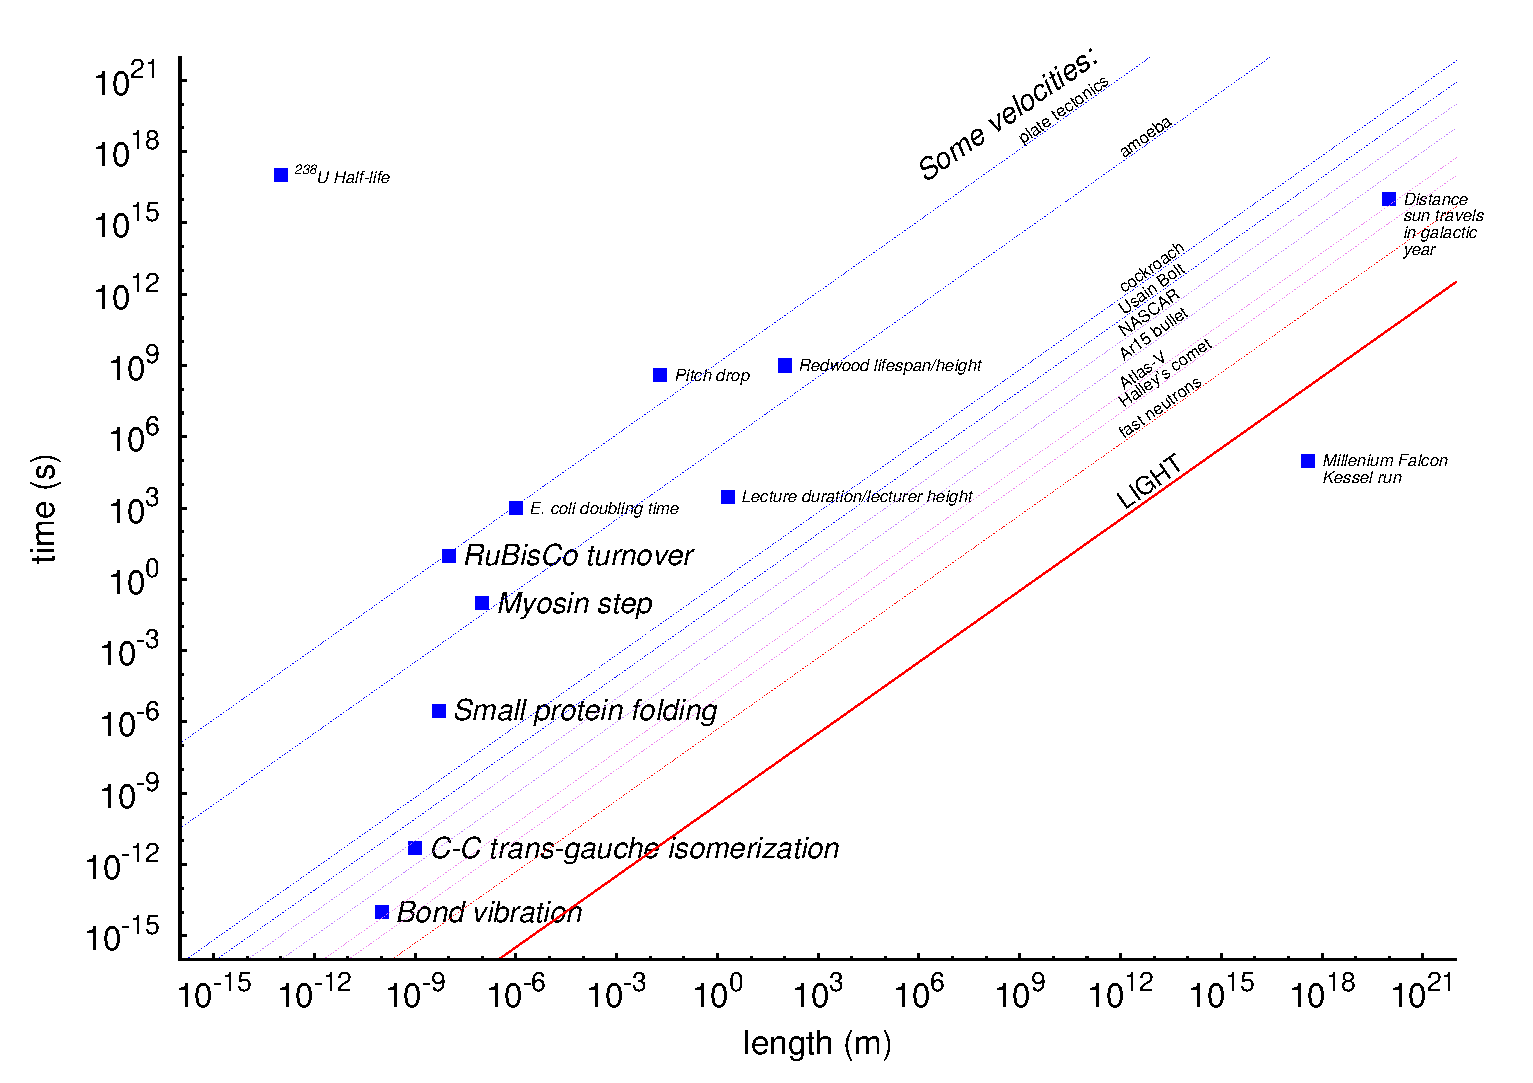
\includegraphics[width=0.975\textwidth]{time_vs_length.eps}};
\begin{scope}[x={(image.south east)},y={(image.north west)}]
\draw[red,thick,rounded corners] (0.2,0.125) rectangle (0.32,0.375);
\draw[red,thick] (0.26,0.275) node {MD};
\draw[->, green!80!black, thick, snake=snake, segment amplitude=.4mm, segment length=2mm, 
line after snake=1mm] (0.29,0.375) -- (0.29,0.45);
\draw[->, green!80!black, thick, snake=snake, segment amplitude=.4mm, segment length=2mm, 
line after snake=1mm] (0.26,0.375) -- (0.26,0.475);
\draw[->, green!80!black, thick, snake=snake, segment amplitude=.4mm, segment length=2mm, 
line after snake=1mm] (0.23,0.375) -- (0.23,0.5);
\draw[->, blue!80!white, thick, snake=snake, segment amplitude=.4mm, segment length=2mm, 
line after snake=1mm] (0.32,0.285) -- (0.38,0.285);
\draw[->, blue!80!white, thick, snake=snake, segment amplitude=.4mm, segment length=2mm, 
line after snake=1mm] (0.32,0.25) -- (0.4,0.25);
\node[green!80!black,text width=2cm,rotate=90] at (0.25,0.65) {Enhanced sampling};
%\draw [red,thick,rotate=-90] (0.3,0.6) node {Enhanced Sampling};
\draw [blue!80!white,thick] (0.57,0.27) node {Resolution coarsening};
\end{scope}
\end{tikzpicture}
\end{frame}



\begin{frame}{The Essential Problem: Poor Sampling of Feature Space}
    \begin{tikzpicture}[scaleall=1.0]
    \pcuad{\textwidth}{\textheight}
    \path(nw) ++(-1,-0.5) node(graphic1)[anchor=north west]{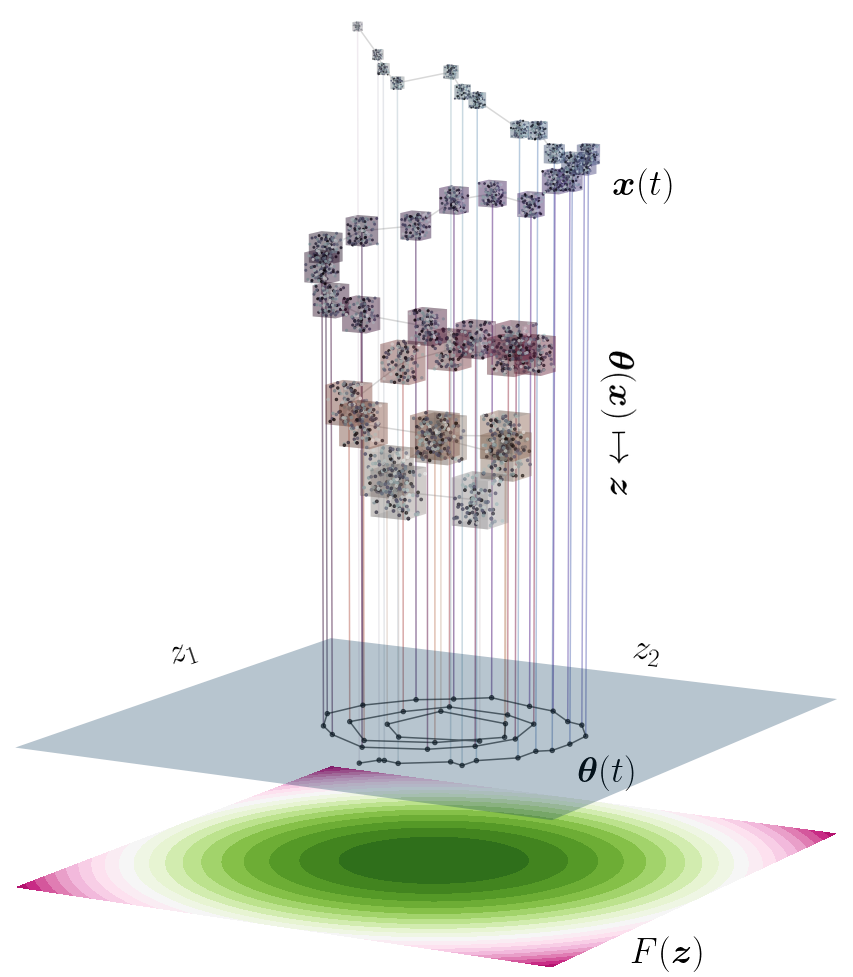
\includegraphics[width=0.6\textwidth]{hmmdfig-crop.png}};
    \path(np) ++(-1,0) node(line1)[anchor=north west]{Configuration space $\xb^{3N} \equiv [(x_0,x_1,x_2)_1,\dots]$}
              ++(0,-1) node(line2)[anchor=west]{MD: $m_i\ddot{x}_i = -\nabla_iV(\xb) + \mbox{ensemble forces}$}
              ++(1,-1) node(line3)[anchor=west]{Samples $\Rightarrow\ \xb(t_1),\ \xb(t_2),\ \dots$}
              ++(0,-1) node(line4)[anchor=west]{Ergodicity: $\displaystyle\langle X\rangle \approx \frac{1}{n_\tau}\sum_{i=1}^{n_\tau} X[\xb(t_i)]$}
              ++(-1.3,-1) node(line5)[anchor=west]{Mapping configuration space}
              ++(0,-0.4) node(line5)[anchor=west]{to feature space}
              ++(0.25,-1.) node(line6)[anchor=west]{Feature space: $\zb^M \equiv (z_1,z_2,\dots)$}
              ++(0,-2) node(line7)[anchor=west]{Free energy: $F(\zb)=-k_{\rm B}T\ln\langle\delta\left[\theta(\xb)-\zb\right]\rangle$};
    \end{tikzpicture}
    \end{frame}
    

\begin{frame}{Hetergeneous Multiscale Molecular Dynamics (HMMD)}
\begin{tikzpicture}[scaleall=1.0]
\pcuad{\textwidth}{\textheight}
\path(nw) ++(-1,-0.5) node(graphic1)[anchor=north west]{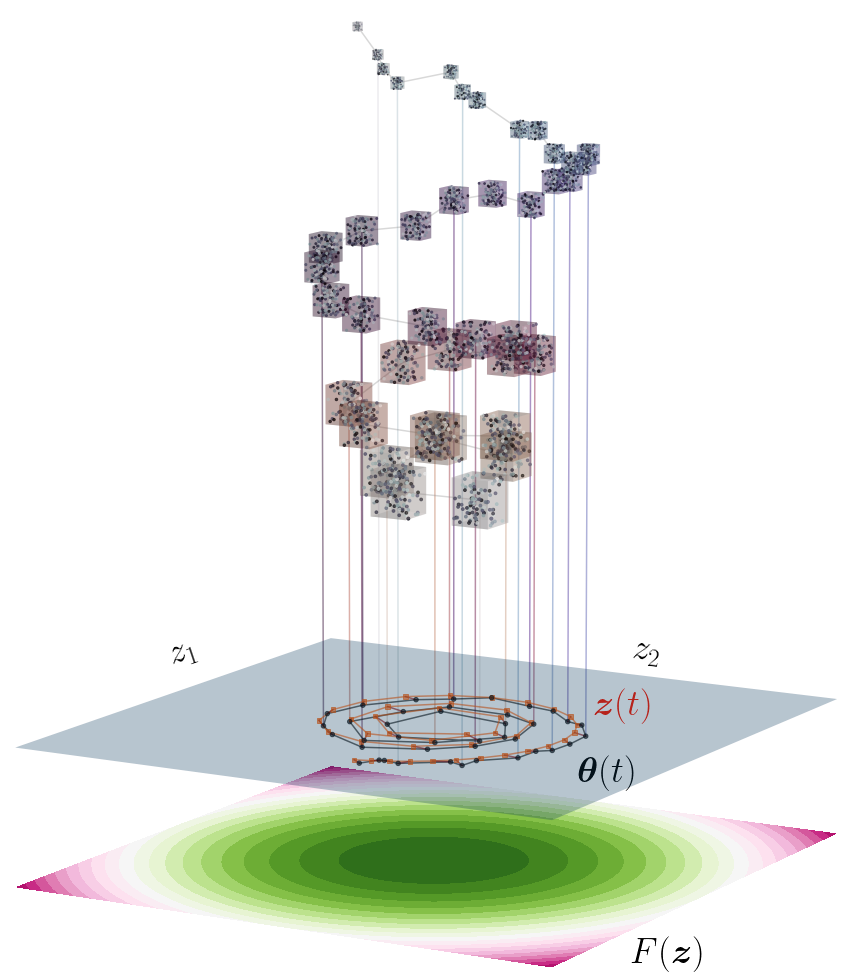
\includegraphics[width=0.6\textwidth]{../hmmdfig2-crop.png}};
\path(np) ++(-1.5,-1) node(line1)[anchor=north west]{Extended configuration space $(\xb^{3N},\ \color{orange!70!black}{\zb^M}\color{black})$}
++(0,-1.5) node(line2)[anchor=west]{$\displaystyle m_i\ddot{x}_i = -\nabla_iV(\xb)-\sum_{j=1}^M\color{green!80!black}{\kappa[\theta_j(\xb)-z_j]}\color{black}\frac{\partial\theta_j}{\partial x_i} + \mbox{e.f.}$}
++(0,-1) node(line3)[anchor=west]{$\displaystyle\bar{m}_j\ddot{z}_j = \sum_{k=1}^{M} \mathcal{M}_{jk}\color{green!80!black}{\kappa[\theta_k(\xb)-z_k]}\color{black} + \color{blue!80!black}{\mbox{bias}}\color{black}$}
++(1,-1.2) node(line4)[anchor=west,align=left] {\textcolor{green!80!black}{Forces} link $\xb$ and $\color{orange!70!black}{\zb}\color{black}$}
++(0,-1) node[anchor=west,align=left,text width=0.6\textwidth] {\textcolor{blue!80!black}{Bias} on $\color{orange!80!black}{\zb}\color{black}$ drives sampling of feature space};
%\draw[] (1.25,2) node {$\thetab(\xb)$};
%\draw[] (2.5,1.75) node {$\zb$};
\end{tikzpicture}
\end{frame}


\section{Temperature-Accelerated MD: Enhanced Feature Sampling}

\begin{frame}[fragile]{Temperature-Accelerated MD}
\vspace{-5mm}
\textcolor{blue}{\tiny Maragliano and Vanden-Eijnden, {\it Chem Phys Lett} {\bf 
426}:168 (2006)}

Extended potential energy:\ \ $\displaystyle U(\xb,\zb) = V(\xb) + 
\frac{1}{2}\kappa\sum_{j=1}^{M}[\theta_j(\xb)-z_j]^2$\\
Dynamics of configurational variables $\xb$ (``restrained MD''):
\begin{displaymath}
m_i\ddot{x}_i = -\frac{\partial V(\xb)}{\partial 
x_i}-\kappa\sum_{j=1}^{M}\left[\theta_j(\xb)-z_j\right]\frac{\partial\theta_j}{
\partial x_i}+\mbox{thermostat @ $\beta$}
\end{displaymath}
Dynamics of auxiliary variables $\zb$ with enforced separation of time-scales:
\begin{displaymath}
\bar\gamma\bar{m}_j\dot{z}_j = \kappa\left[\theta_j(\xb)-z_j\right] + 
(\mbox{noise @ $\bar\beta$}) \approx -\frac{\partial F}{\partial z_j} + 
\mbox{noise}
\end{displaymath}

$\zb$ responds to free energy like $\xb$ responds to potential energy.\\
Taking $\bar\beta < \beta$ ($\bar{T} > T$)\ $\Rightarrow$\ enhanced sampling in 
a chosen feature space.

\end{frame}



\begin{frame}[fragile]{TAMD predicts HIV-1 gp120 conformational changes}
\begin{tikzpicture}
\pcuad{\textwidth}{\textheight}
\path(nw) ++(-0.75,0.0) node(text)[anchor=north west,text width=\textwidth]{{\tiny \textcolor{red!80!black}{CFA and E. Vanden-Eijnden {\it PNAS} {\bf 107}:4961 (2010).}}} ++(0,-0.33) node(topfig)[graphics,anchor=north west]{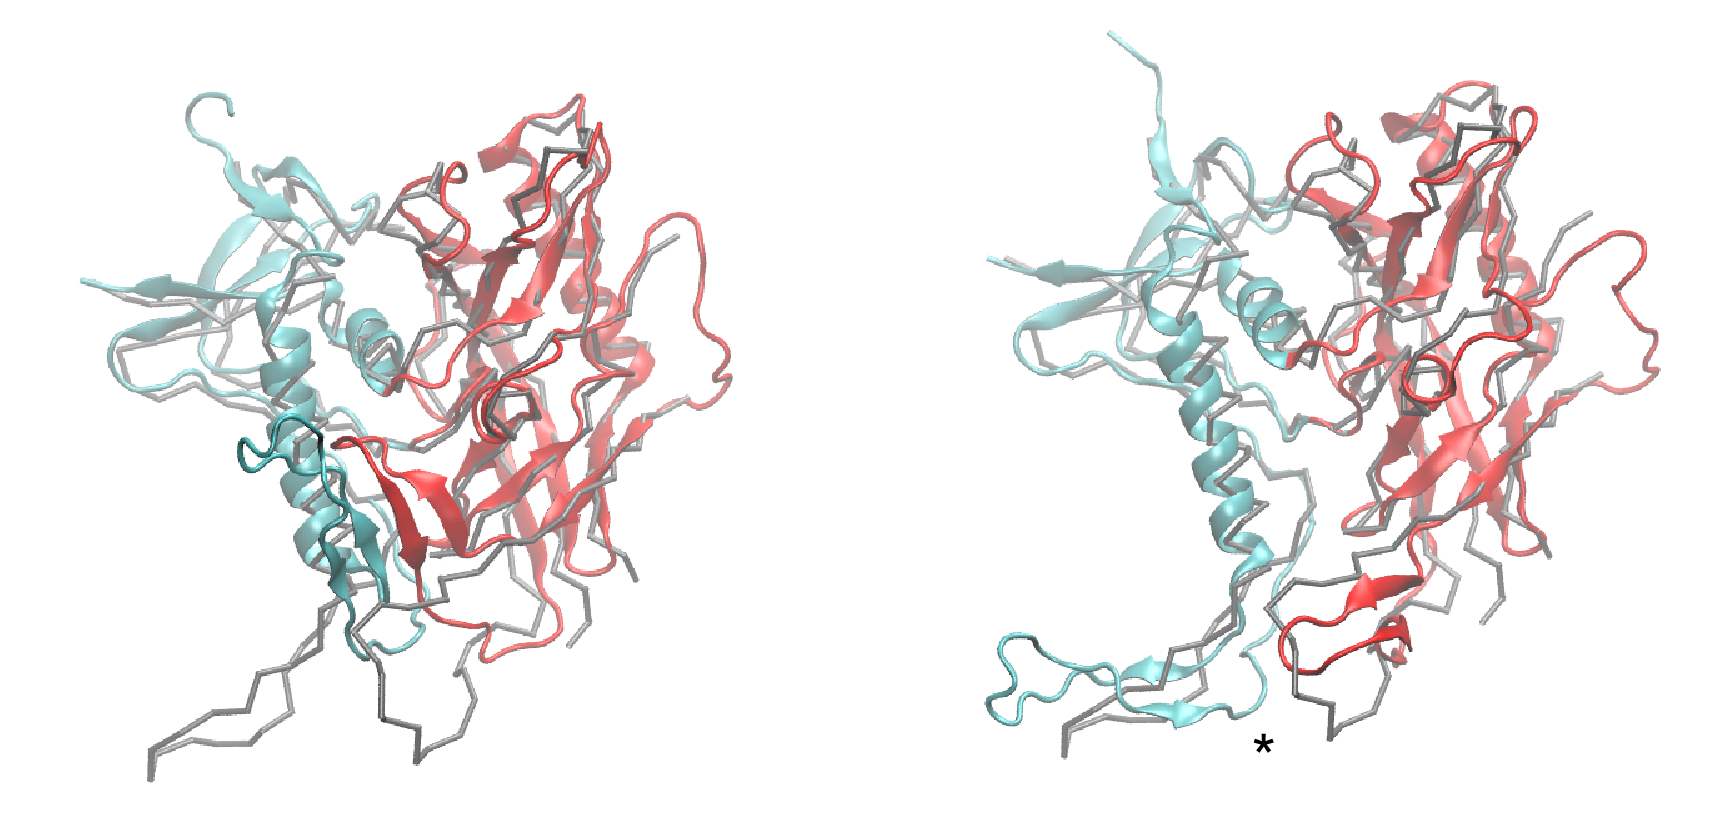
\includegraphics[width=0.8\textwidth]{gp120_snap.png}} ++(0,-4) node(botfig)[graphics,anchor=north west]{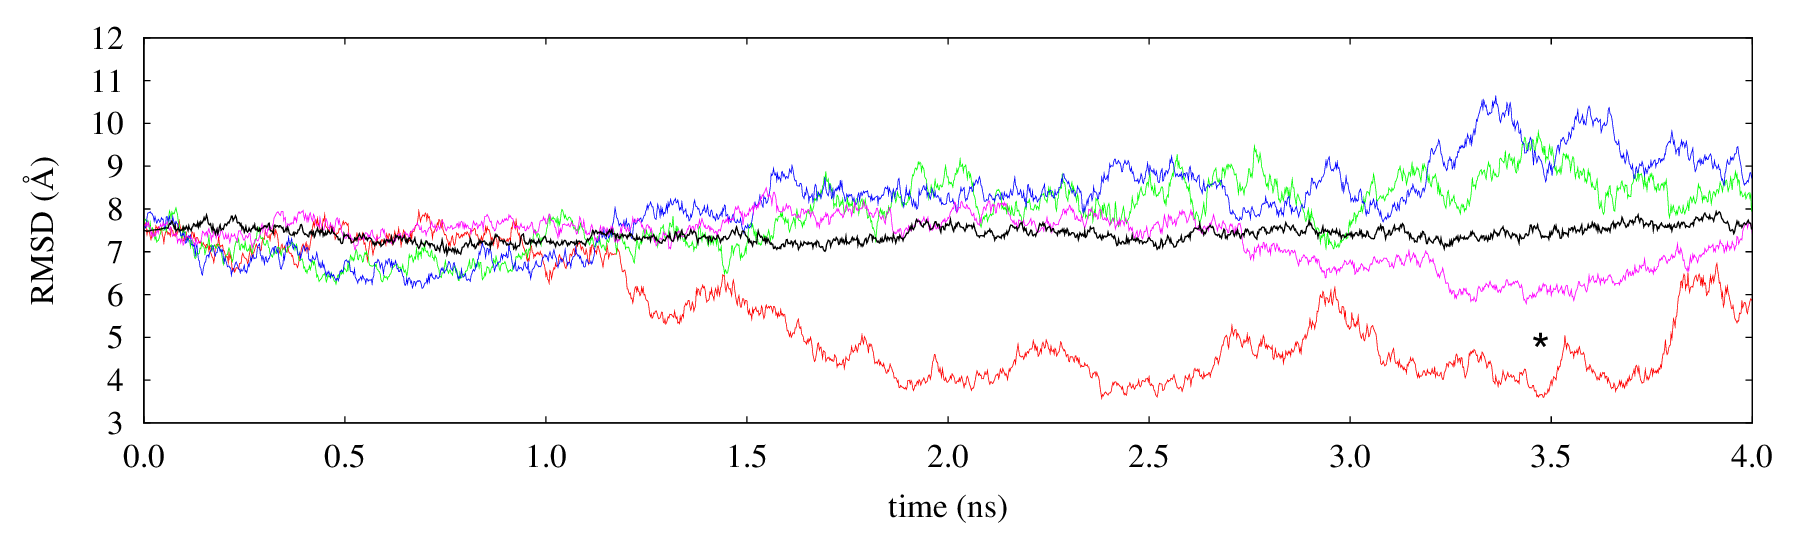
\includegraphics[width=\textwidth]{gp120_rmsdplot.png}}; 
\path(ne) ++(0,0) node(text2)[anchor=north east,text width=0.3\textwidth]{
\begin{itemize}
\item Ribbon: TAMD from 1GC1 (ground state) (\textcolor{teal}{inner}/\textcolor{red}{outer})
\item Tube: Reference from 3HI1 (Ab-F105-bound)
\end{itemize}};
\end{tikzpicture}
\end{frame}



\section{On-the-Fly Parameterization:  Free-Energy Calculations}

\begin{frame}[fragile]{On-the-Fly Parameterization (OTFP) to Get $F$ from TAMD}
    \begin{tikzpicture}
        \pcuad{\textwidth}{\textheight}
        %\showcuad
        \path(se) 
            ++(0,1) node(text)[anchor=south east]{
                {\tiny \textcolor{blue!80!black}{CFA and E. Vanden-Eijnden {\em Chem Phys Lett} {\bf 547}:114 (2012)}}
            };
        \path(nw) 
            ++(0,-0.5) node(text)[anchor=west]{
                \textcolor{blue!80!black}{Basis-function expansion}
            }
            ++(0,-0.75) node(Fz)[anchor=west]{
                $\ds \tilde{F}(\zb) = \sum_k\lambda_k\phi_k(\zb)$
            }
            ++(0,-1) node(text2)[anchor=west]{
                \textcolor{red!80!black}{Error estimate}
            }
            ++(0,-0.8) node(Elambda)[anchor=west]{
                $\ds E(\lambdab) = \Big<\sum_j\left[\kappa[z_j-\theta_j(\xb)]-\frac{\partial \tilde{F}(\zb)}{\partial 
        z_j}\right]^2\Big>_{\rm TAMD}$
            }
            ++(3,1.25) node(min)[anchor=west]{
                \textcolor{green!80!black}{Minimize}
            }
            ++(1.5,1) node(dEdlambda)[anchor=west]{
                $\ds \frac{\partial E}{\partial \lambdab}=0$
            }
            ++(1.75,0) node(A)[anchor=west]{
                $\ds \uu{A}\lambdab = \uu{b}$
            }
            ++(1.75,0) node(lam)[anchor=west]{
                $\ds\lambdab = \uu{A}^{-1}\uu{b}$
            }
            ++(2.25,0) node(FF)[anchor=west]{
                $\ds \tilde{F}(\zb)$
            };
        \draw [->,thick,color=orange!80!black] (Elambda.north) -- (min.south);
        \draw [->,thick,color=orange!80!black] (min.north) -- (dEdlambda.south west);
        \draw [->,thick,color=orange!80!black] (dEdlambda.east) -- (A.west);
        \draw [->,thick,color=orange!80!black] (A.east) -- (lam.west);
        \draw [->,thick,color=orange!80!black] (lam.east) -- (FF.west);
        \path(wp) 
            ++(0,0) node(Anm)[anchor=west]
            {
                {\tiny $\ds A_{nm} = \frac{1}{2}\left<\sum_i\frac{\partial \phi_m(\zb)}{\partial z_i} 
        \frac{\partial \phi_n(\zb)}{\partial z_i}\right>_{\rm TAMD}$}
            }
            ++(0,-0.7) node(bm)[anchor=west]{
                {\tiny $\ds b_{m} = \left<\sum_i\frac{\partial \phi_m(\zb)}{\partial 
        z_i} \kappa[z_i-\theta_i(\xb)]\right>_{\rm TAMD}$}
            };
        
        \draw[<->,thick,color=green!80!black] (0.1\bbw,0.2\bbh) -- (0.5\bbw,0.2\bbh);
        \draw[->,thick,color=green!80!black] (0.3\bbw,0.2\bbh) -- (0.3\bbw,0.35\bbh);
        \draw[thick,color=orange!50!black] (0.4\bbw,0.2\bbh) -- (0.3\bbw,0.3\bbh);
        \draw[thick,color=orange!50!black] (0.3\bbw,0.3\bbh) -- (0.2\bbw,0.2\bbh);
        \draw[thick,color=green!80!black] (0.2\bbw,0.2\bbh) -- (0.2\bbw,0.18\bbh);
        \draw[thick,color=green!80!black] (0.4\bbw,0.2\bbh) -- (0.4\bbw,0.18\bbh);
        \draw[thick,color=green!80!black] (0.3\bbw,0.2\bbh) -- (0.3\bbw,0.18\bbh);
        \draw (0.3\bbw,0.15\bbh) node {$m$};
        \draw (0.2\bbw,0.15\bbh) node {$m-1$};
        \draw (0.4\bbw,0.15\bbh) node {$m+1$};
        \draw (0.32\bbw,0.32\bbh) node {1};
        \draw (0.35\bbw,0.29\bbh) node {$\phi_m$};
        
        \path(ep) 
            ++(0,0.5) node(plot)[graphics,anchor=north east]{
                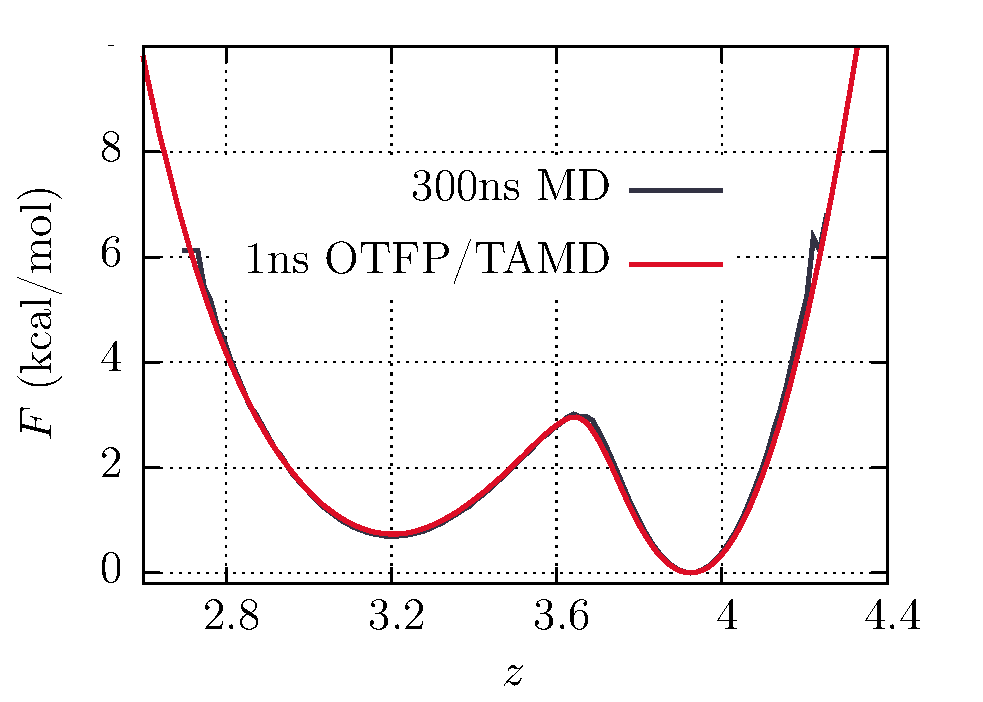
\includegraphics[width=0.45\textwidth]{otfpc4}
            }
            ++(0,0) node(config)[graphics,anchor=south east]{
                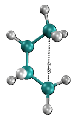
\includegraphics[width=0.16\textwidth]{butane}
            };
        \end{tikzpicture}
\end{frame}



\begin{frame}[fragile]{DAVEI: Dual-Acting Virolytic Entry Inhibitors}
\begin{tikzpicture}[scaleall=1.0]
\pcuad{\textwidth}{\textheight}
%\showcuad
\path(nw) ++(-0.75,0.15) node(text)[anchor=north west,text 
width=1.1\textwidth]{{\tiny \textcolor{red!80!black}{Contarino, Bastian, Sundaram, McFadden, Duffy, Gangupomu, Baker, Abrams, Chaiken, {\it Antimicrob.
 Agents Chemother.} 2013, {\bf 57}:4743\\*[-1em]
Parajuli, Acharya, Yu, Ngo, Rashad, Abrams, Chaiken, {\it Biochemistry} 2016 {\bf 55}:6100}}};
\path(nw) ++(-1,-1) node(text2)[anchor=north west,text width=1.1\textwidth]{
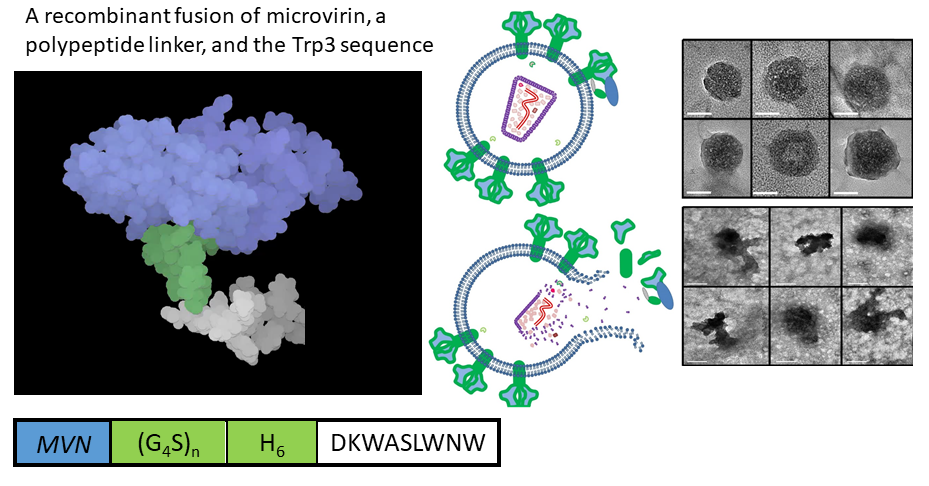
\includegraphics[width=\textwidth]{davei_whatisit.png}};
\end{tikzpicture}
\end{frame}


% asparagines: 262 dash
% 332 dot
% 386 dash dot-dot
% 392 long-dash dot
% 448 solid
\begin{frame}[fragile]{OTFP Predicts DAVEI Activity Dependence on Linker Length}
\begin{tikzpicture}[scaleall=1.0]
\pcuad{\textwidth}{\textheight}
%\showcuad
\path(nw) ++(-0.75,0.15) node(text)[anchor=north west,text 
width=\textwidth]{{\tiny \textcolor{red!80!black}{S. Gossert and CFA, {\it Protein Science}, vol. 29, pp. 2304-2310, 2020. doi:10.1002/pro.3949}}};
\path(nw) ++(-0.75,-4) node(text2)[anchor=north west,text width=0.5\textwidth]{
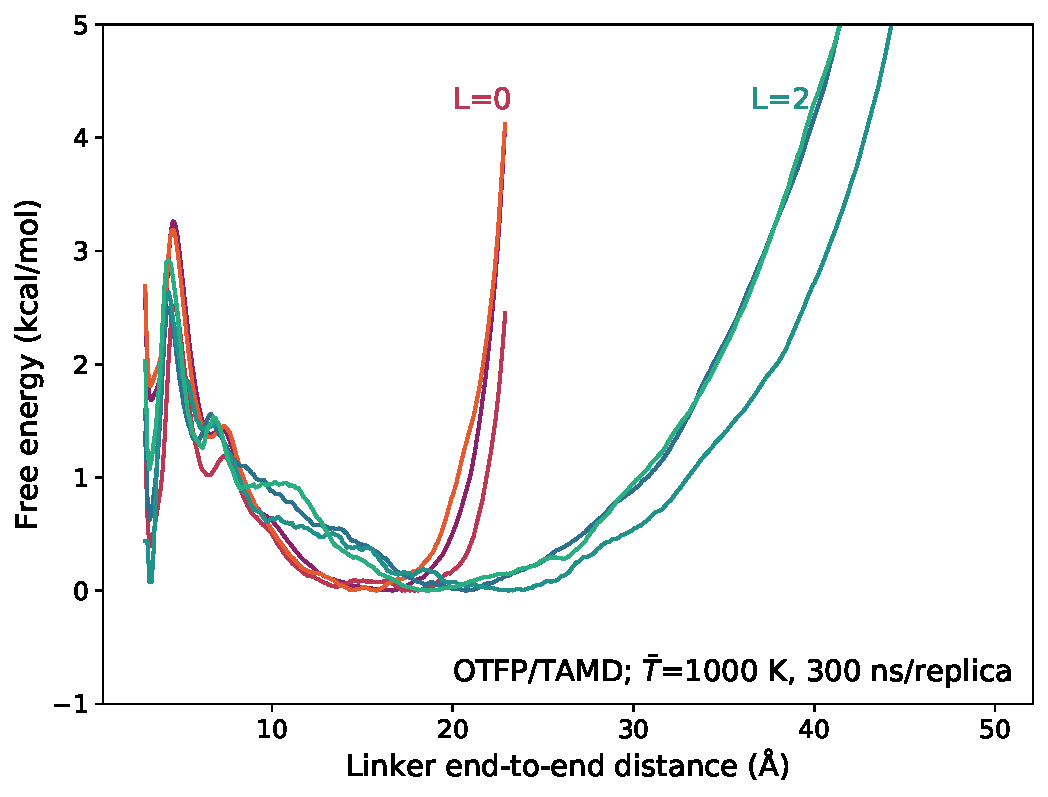
\includegraphics[width=\textwidth]{linker_pmf.pdf}};
\path(nw) ++(0.5,-0.15) node(text2)[anchor=north west,text width=0.4\textwidth]{
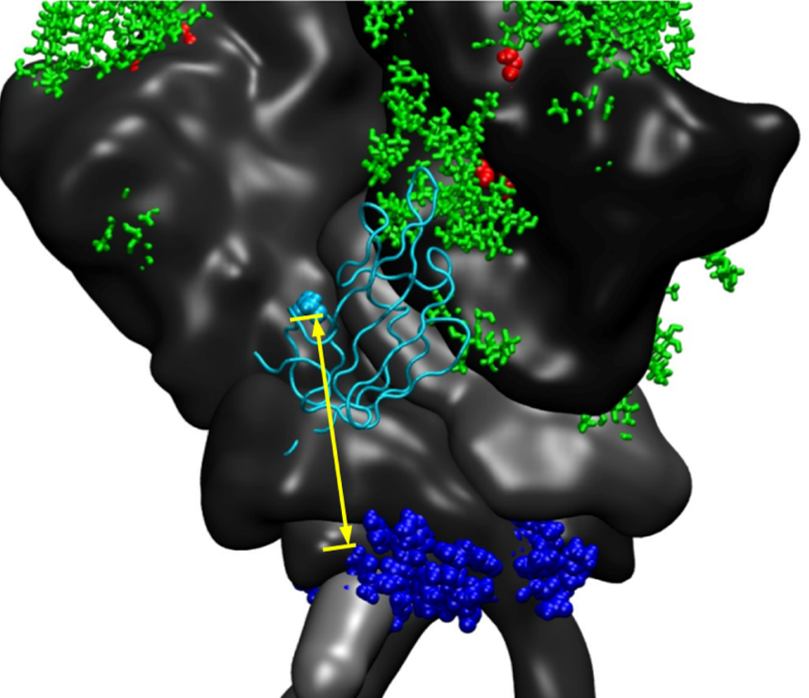
\includegraphics[width=\textwidth]{env+mvn_dist.png}};
\path(nw) ++(5,0) node(text2)[anchor=north west,text width=0.6\textwidth]{
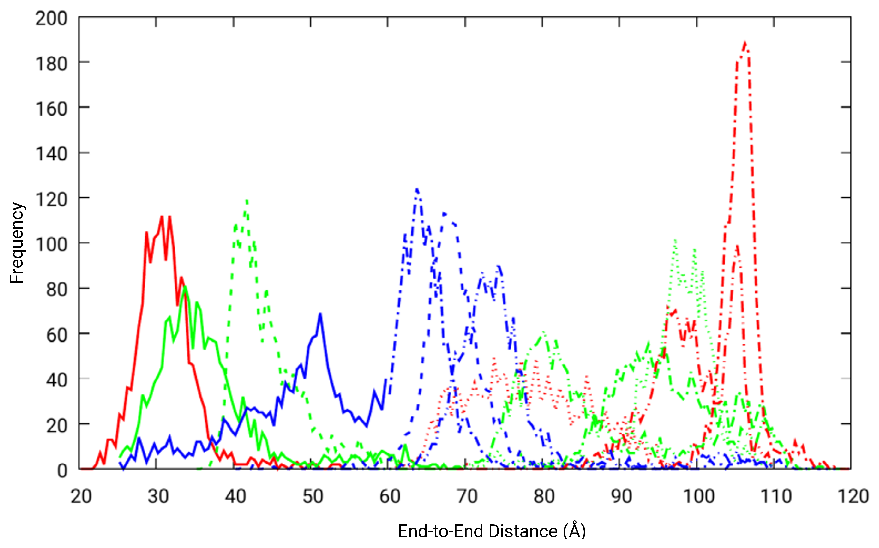
\includegraphics[width=\textwidth]{davei_env_mvn_dist_hist_1.png}};
\path(nw) ++(5.75,-0.25) node(text3)[anchor=north west,text width=0.5\textwidth]{\tiny MD, 40 ns};
\path(nw) ++(5.5,-4.25) node(text2)[anchor=north west,text width=0.45\textwidth]{
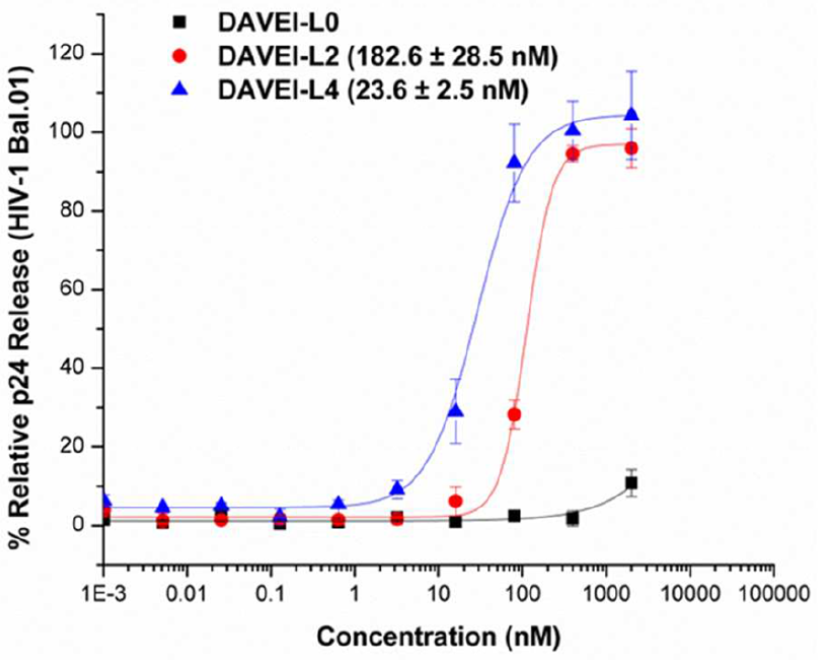
\includegraphics[width=\textwidth]{DAVEI-L02-experiment.png}};
\path(nw) ++(6.5,-0.5) node(text2)[anchor=north west,text width=0.1\textwidth]{
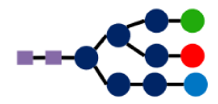
\includegraphics[width=\textwidth]{man9.png}};
\path(nw) ++(8.5,-0.4) node(text2)[anchor=north west,text width=0.08\textwidth]{
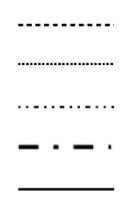
\includegraphics[width=\textwidth]{dashkey.png}};
\path(nw) ++(8.5,-0.25) node(text3)[anchor=north west,text width=0.5\textwidth]
{\tiny N-linked glycans};
\path(nw) ++(8.5,-0.4) node(text3)[anchor=north west,text width=0.5\textwidth]
{\tiny 262};
\path(nw) ++(8.5,-0.66) node(text3)[anchor=north west,text width=0.5\textwidth]
{\tiny 332};
\path(nw) ++(8.5,-0.92) node(text3)[anchor=north west,text width=0.5\textwidth]
{\tiny 386};
\path(nw) ++(8.5,-1.18) node(text3)[anchor=north west,text width=0.5\textwidth]
{\tiny 392};
\path(nw) ++(8.5,-1.48) node(text3)[anchor=north west,text width=0.5\textwidth]
{\tiny 448};
\path(nw) ++(-0.75,-1.5) node(label1)[anchor=north west,text width=0.4\textwidth]{MVN at\\N448 glycan};
\path(nw) ++(0.6,-2.4) node(label2)[anchor=north west,text width=0.2\textwidth]{40 \AA};
\path(nw) ++(-0.2,-3.2) node(label3)[anchor=north west,text width=0.4\textwidth]{Trp3 at MPER};
\end{tikzpicture}
\end{frame}



\begin{frame}[fragile]{Potassium Channels}
\begin{tikzpicture}[scaleall=1.0]
\pcuad{\textwidth}{\textheight}
%\showcuad
\path(nw) ++(-0.5,0.25) node(corner)[graphics,anchor=north 
west]{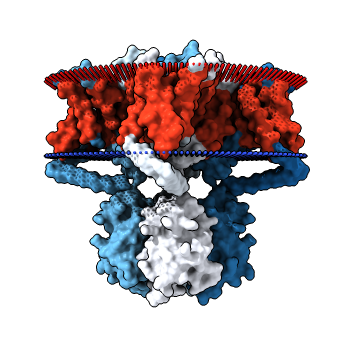
\includegraphics[width=0.33\textwidth]{2a79.png}};
\path(wp) ++(-0.0,1.0) node(corner)[graphics,anchor=north 
west]{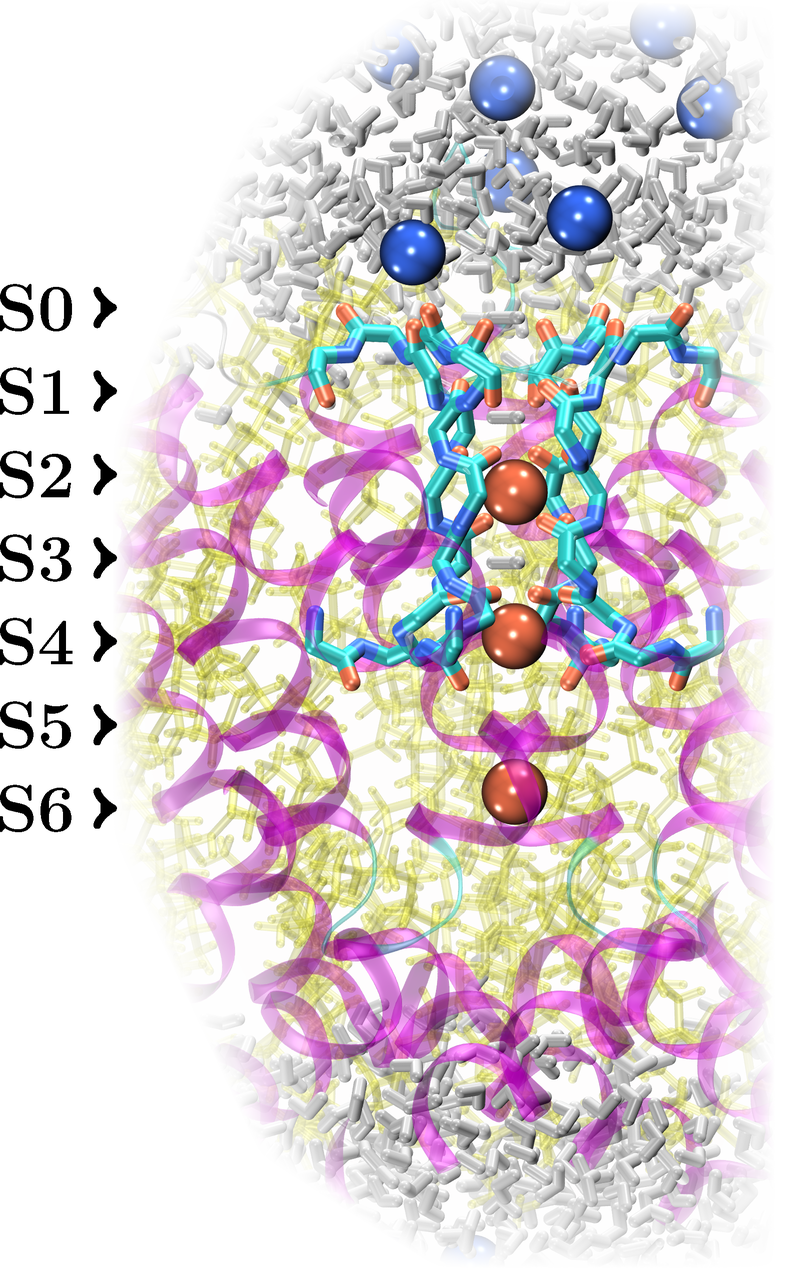
\includegraphics[width=0.25\textwidth]{Kv12_sfilter.png}};
\path(nw) ++(3,0) node(text)[anchor=north west,text width=0.75\textwidth]{
\begin{itemize}
\item Responsible for cell membrane {\em depolarization} in action-potential firing
\item Malfunctions: ``channelopathies'' like episodic ataxia, neuromyotonia, seizure, and tinnitus
\item Selectivity mechanism is not well-understood because the selectivity filter is complicated
\end{itemize}
};
\path(wp) ++(3.5,0.0) node(plot)[graphics,anchor=north west]{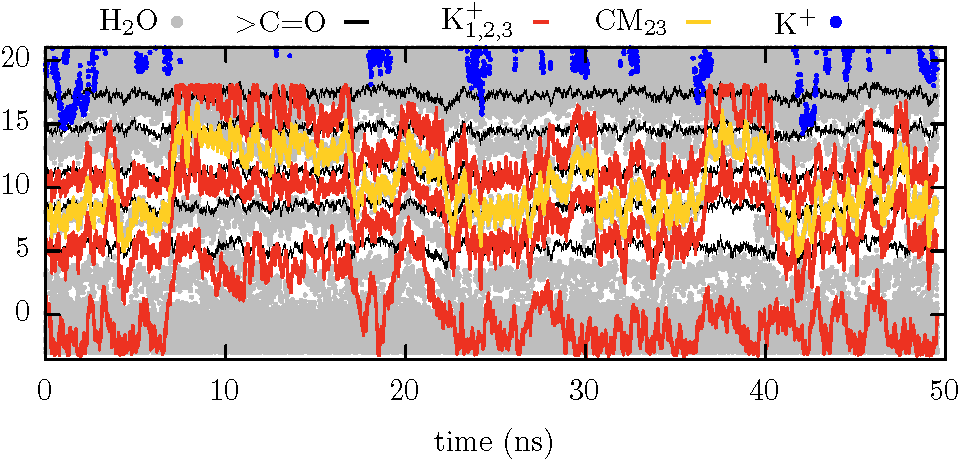
\includegraphics[width=0.65\textwidth]{fullions-crop.png}};
\path(nw) +(0,0.2) node(cite)[anchor=north west]{\tiny \textcolor{red!80!black}{S. A. Paz, L. Maragliano, and CFA {\em J. Chem. Theory. Comput.} {\bf 14}:2743-2750 (2018)}};
\end{tikzpicture}

\end{frame}



\begin{frame}{2D OTFP: Transport Minimum Free-Energy Pathways}
\begin{tikzpicture}
\pcuad{\textwidth}{\textheight}
%\showcuad
\path(nw) +(0,0.2) node(cite)[anchor=north west]{\tiny \textcolor{red!80!black}{S. A. Paz, L. Maragliano, and CFA {\em J. Chem. Theory. Comput.} {\bf 14}:2743-2750 (2018)}};
\path(nw) +(0,0) node(image)[anchor=north west]{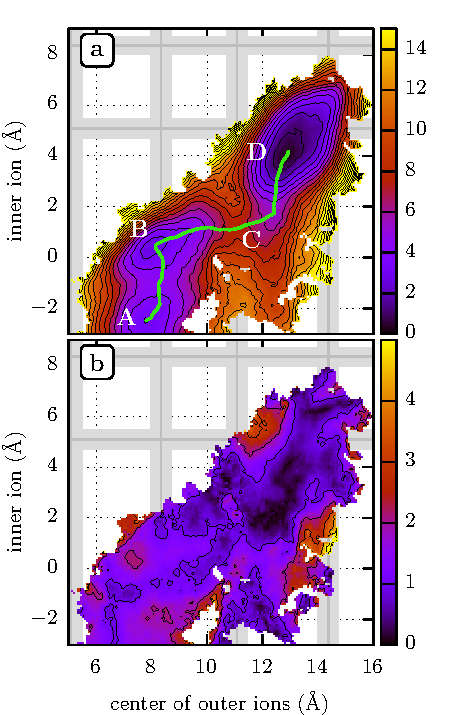
\includegraphics[width=0.5\textwidth]{fullfes_path_err.pdf}};
\path(nw) +(1.5,-4) node(errlab)[anchor=north west]{Error, $N$=3};
\path(nw) +(5,-1.5) node(bullets)[anchor=north west,text width=0.5\textwidth]{\begin{itemize}
\item A$\rightarrow$B: Innermost ion moves up one position
\item B$\rightarrow$C: CM$_{2,3}$ moves up one position, followed quickly by
\item C$\rightarrow$D: Innermost ion moves up one more position
\item $\Rightarrow$ Net translocation of one K$^+$
\item What role is water playing?
\end{itemize}};
\end{tikzpicture}
\end{frame}



\begin{frame}{Water Restraints: Ion-Tethered vs. Excluded-from-Filter}
\begin{tikzpicture}
\pcuad{\textwidth}{\textheight}
%\showcuad
\path(nw) +(0,0) node(image)[anchor=north west]{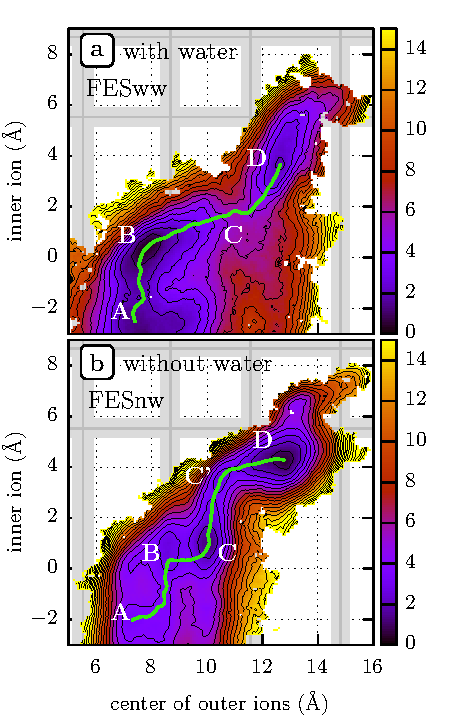
\includegraphics[width=0.5\textwidth]{wc_fes.pdf}};
\path(nw) +(5,-1.5) node(bullets)[anchor=north west,text width=0.5\textwidth]{\begin{itemize}
\item With one water tethered to each K$^+$, FES resembles unrestrained one
\item With water excluded from channel, ion motion is less concerted, more ``hard-knock'' like
\end{itemize}};
\end{tikzpicture}
\end{frame}



%\begin{frame}{Free-Energy Profiles along MFEP's}
\begin{tikzpicture}
\pcuad{\textwidth}{\textheight}
%\showcuad
\path(nw) +(0,0.2) node(cite)[anchor=north west]{\tiny \textcolor{red!80!black}{S. A. Paz, L. Maragliano, and CFA {\em J. Chem. Theory. Comput.} {\bf 14}:2743-2750 (2018)}};
\path(np) +(0,0) node(image)[anchor=north]{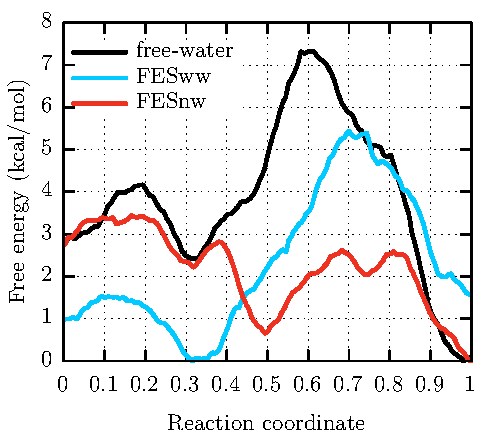
\includegraphics[width=0.67\textwidth]{paths.pdf}};
\path(nw) +(0,-6) node(bullets)[anchor=north west,text width=\textwidth]{\begin{itemize}
\item Energy barriers for unrestricted and ion-tethered water systems are similar; suggests intercalated water is preferred
\item Dry filter shows shallower barriers; dry transport might be faster if water could be actively excluded
\end{itemize}};
\end{tikzpicture}
\end{frame}



\section{The String Method in Collective Variables: Reversible Pathways}

\begin{frame}{String Method in Collective Variables (SMCV)}
\begin{tikzpicture}
\pcuad{\textwidth}{\textheight}
\path(nw) 
    ++(0,-0.5) node(title1)[anchor=north west,text width=\textwidth]{
        \nohyphens{A convergent approach to find \textcolor{red!80!black}{minimum free-energy (reversible) pathways} in feature space represented by sequences of system {\bf images}}
    }
    ++(0,-0.1\bbh) node(graphic1)[anchor=north west]{
        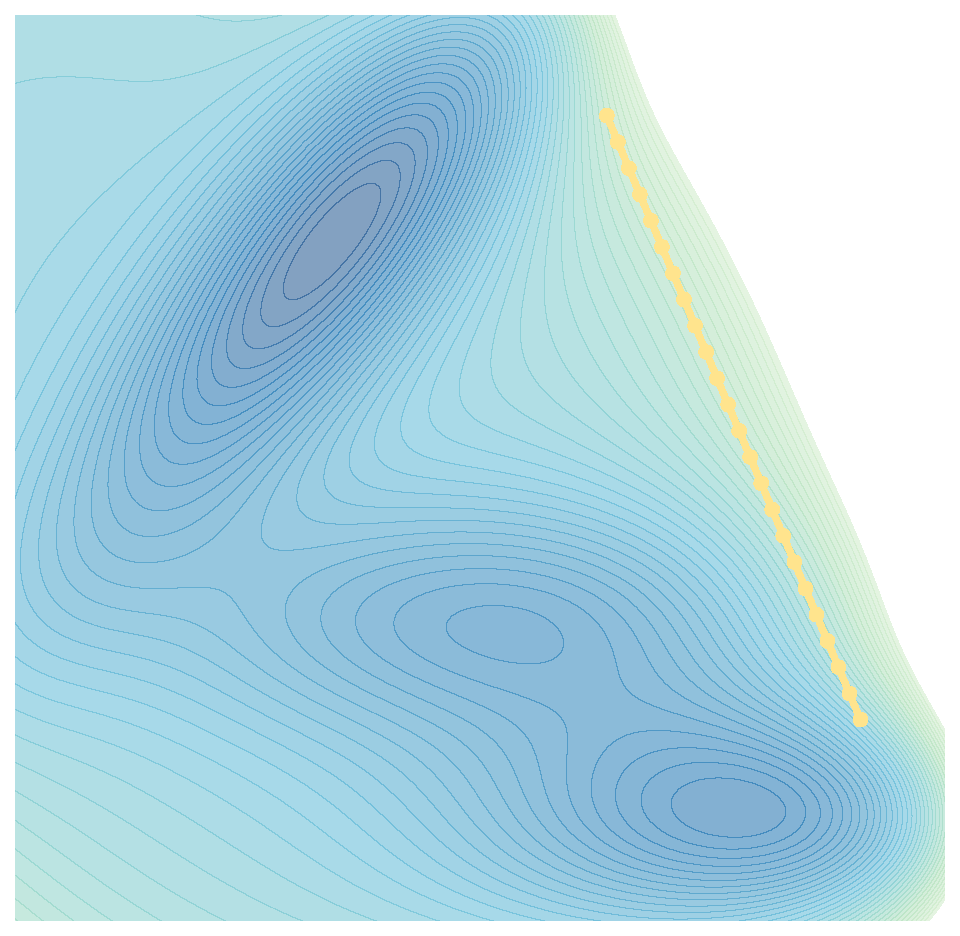
\includegraphics[width=0.25\textwidth]{sm0.pdf}
    }
    ++(0.25\bbw,0) node(graphic2)[anchor=north west]{
        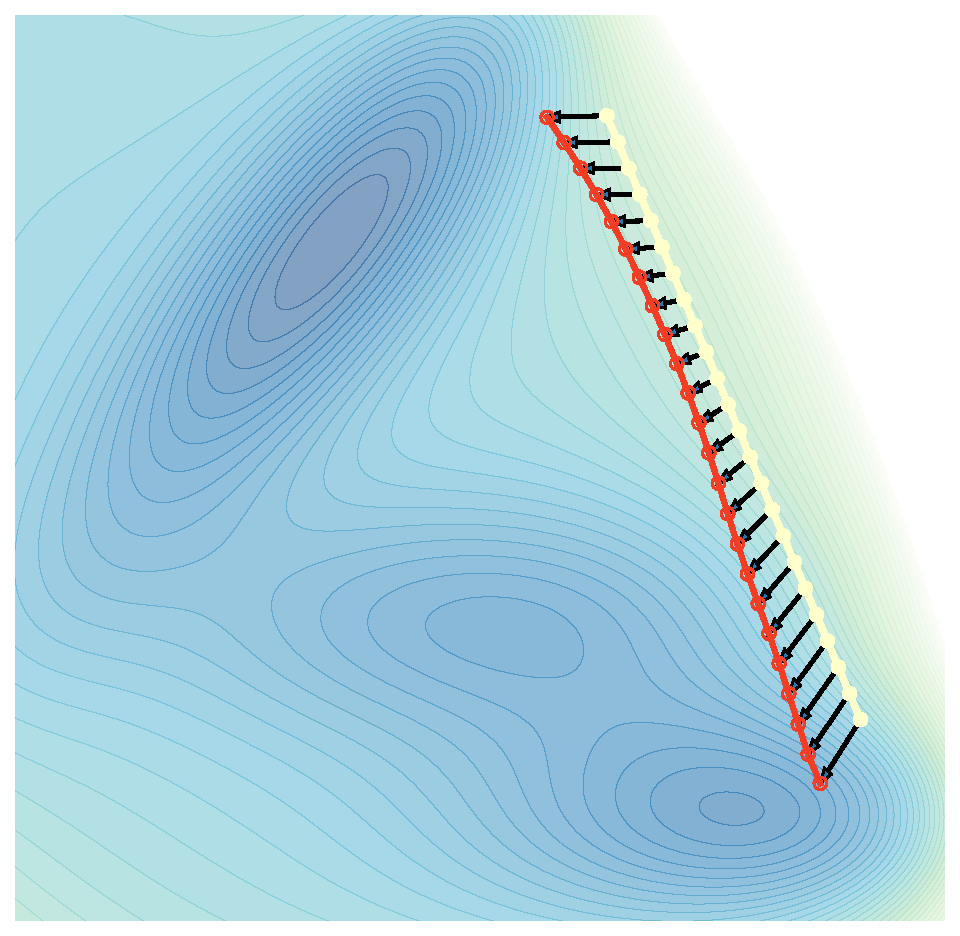
\includegraphics[width=0.25\textwidth]{sm1.pdf}
    }
    ++(0.25\bbw,0) node(graphic3)[anchor=north west]{
        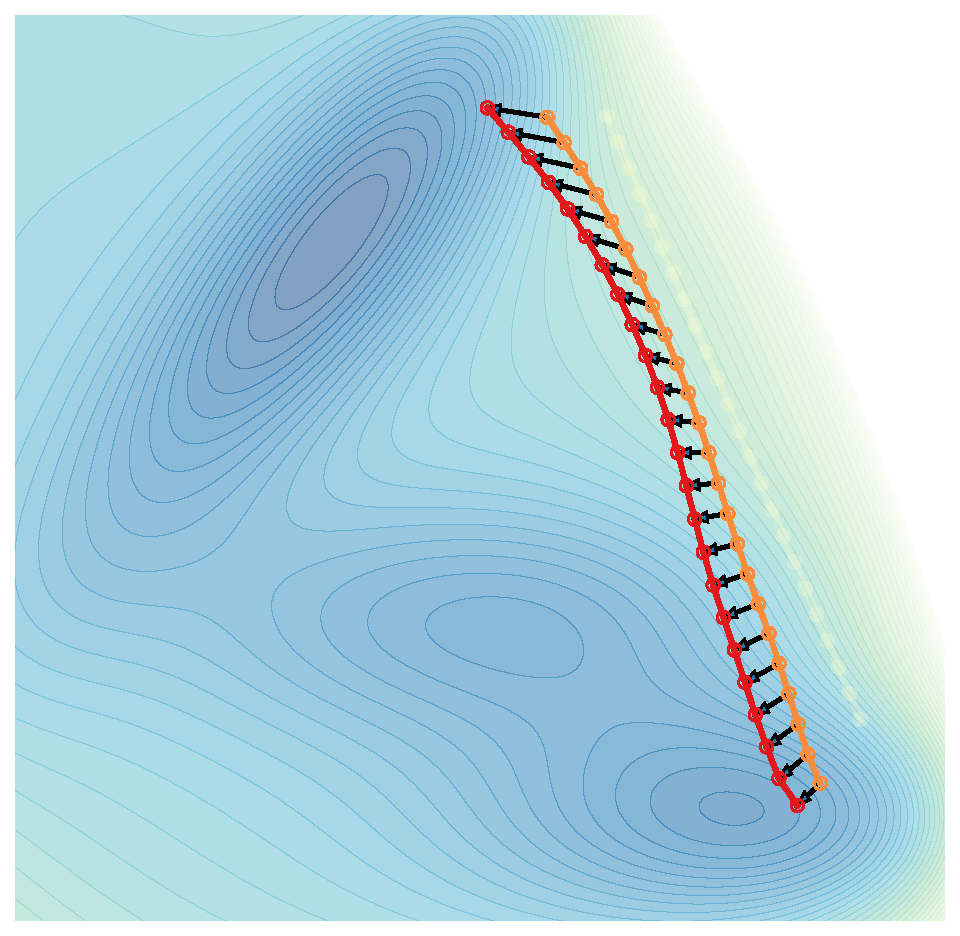
\includegraphics[width=0.25\textwidth]{sm2.pdf}
    }
    ++(0.25\bbw,0) node(graphic4)[anchor=north west]{
        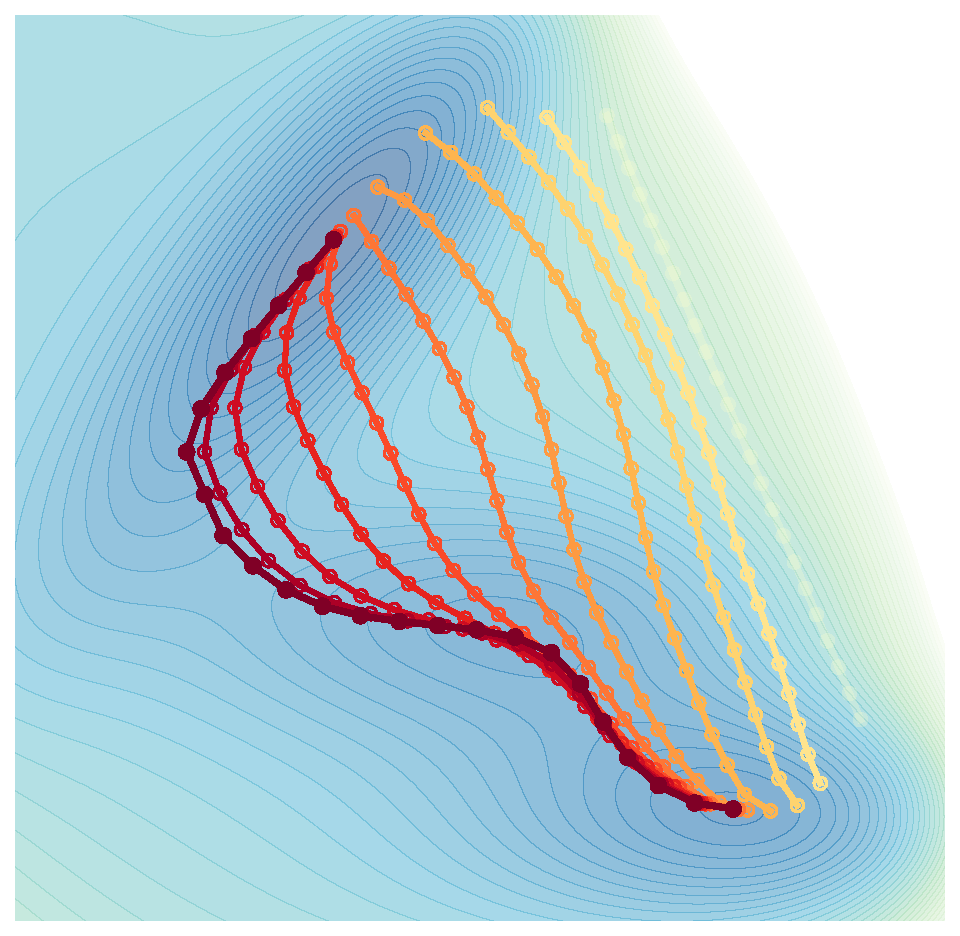
\includegraphics[width=0.25\textwidth]{sm3.pdf}    
    };
\path(cp) 
    ++(0,0) node(label1)[anchor=north]{
        Initial image positions: 
        $\left\{\zb\right\}(0)\equiv\left\{\zb_1(0),\zb_2(0),\dots,\zb_M(0)\right\}$
    }
    ++(0,-0.06\bbh) node(label2)[anchor=north]{
        Image updates: 
        $\left\{\zb\right\}(t+\Delta t)=\left\{\zb\right\}(t)-\Delta t\frac{\displaystyle\partial F}{\displaystyle\partial\left\{\zb\right\}}+\mbox{reparam.}$
    }
    ++(0,-0.12\bbh) node(label3)[anchor=north]{
        Mean forces on image 
        $i$: $-\frac{\displaystyle\partial F}{\displaystyle\partial\zb_i}=\langle\kappa\left[\thetab_i(\xb_i)-\zb_i\right]\rangle_{\zb_i}$
    }
    ++(0,-0.12\bbh) node(label4)[anchor=north]{
        found by restrained MD: 
        $\displaystyle\langle\kappa\left[\thetab_i(\xb_i)-\zb_i\right]\rangle_{\zb_i}=\frac{1}{N_{s}}\sum_{j=1}^{N_s}\kappa\left\{\thetab_i[\xb_i(t_j^{MD})]-\zb_i\right\}$
    };
\end{tikzpicture}
\end{frame}


\begin{frame}{Climbing Strings and Climbing Multistrings}
\begin{tikzpicture}[scaleall=1.0]
\pcuad{\textwidth}{\textheight}
\path(nw) 
    ++(0,-0.5) node(graphic1)[anchor=north west]{
        \nohyphens{Identify nearest \textcolor{red!80!black}{saddle points} to a free-energy minimum in feature space}
    }
    ++(0,-1) node(graphic1)[anchor=north west]{
        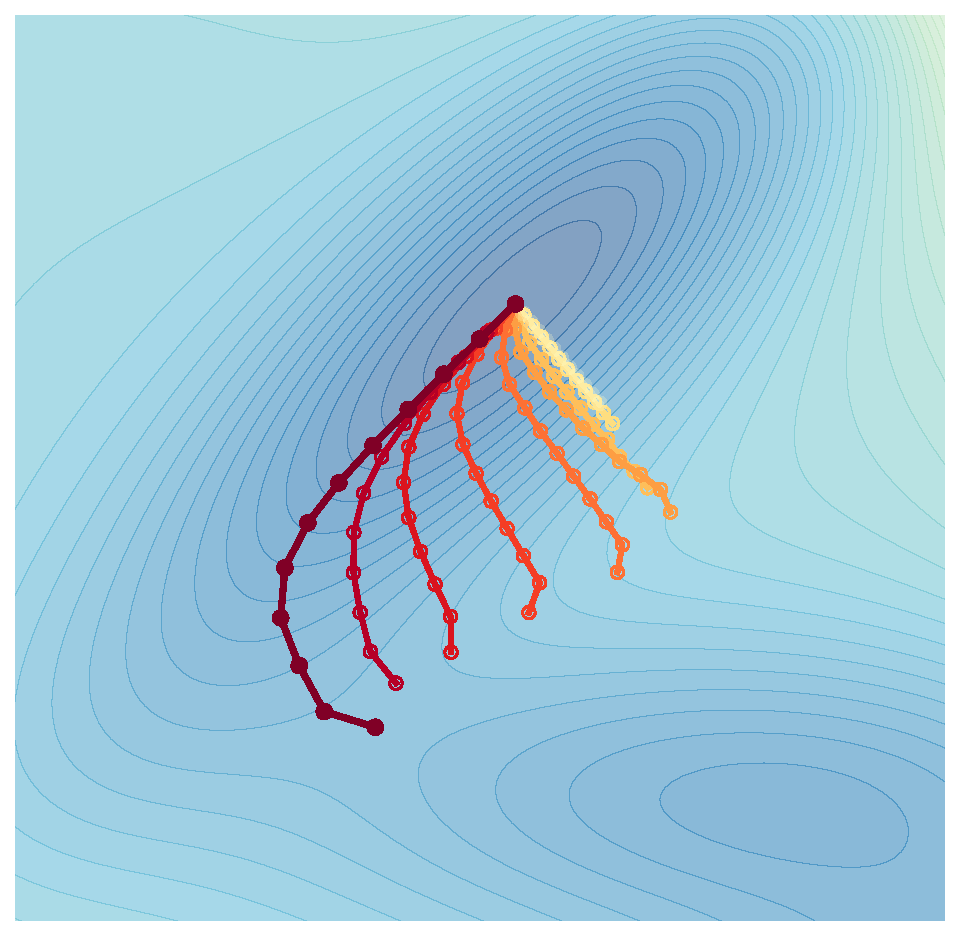
\includegraphics[width=0.5\textwidth]{csm.pdf}
    }
    ++(0.6\bbw,-0.5) node(eqns)[anchor=north west,text width=0.4\textwidth]{
        \nohyphens{Climbing image has force reversed along tangent $\hat{\taub}$}
    }
    ++(0,-1.5) node(lab1)[anchor=north west]{
        $\zb_N^\prime(t) = \zb_N(t) - \nu\ d\zb\cdot\hat{\taub}$
    }
    ++(0,-1) node(lab2)[anchor=north west]{
        $d\zb \equiv \zb_N(t) - \zb_N(t-\Delta t)$
    }
    ++(0,-1) node(lab3)[anchor=north west]{
        $\nu > 1$: friction parameter
    };
\end{tikzpicture}
\end{frame}

\begin{frame}{Climbing Multistrings}
\begin{tikzpicture}[scaleall=1.0]
\pcuad{\textwidth}{\textheight}
\path(nw) 
    ++(0,0) node(header)[anchor=north west]{
        \nohyphens{Systematically search out \textcolor{red!80!black}{all} saddles connected to a minimum}
    }
    ++(0,-0.6) node(graphic1)[anchor=north west]{
        \animategraphics[loop,controls,width=0.5\textwidth]{10}{../movie1/cms1-}{0}{36}
    }
    ++(0.5\textwidth,0) node(graphic2)[anchor=north west]{
        \animategraphics[loop,controls,width=0.5\textwidth]{10}{../movie2/cms2-}{0}{68}
    };
\path(graphic1.south west)
    ++(0,-0.6) node(label1)[anchor=west]{
        Simultaneous independent climbers
    };
\path(graphic2.south west)
    ++(0,-0.6) node(label2)[anchor=west]{
        Simultaneous \textcolor{red!80!black}{interacting} climbers
    };
\path(se)
    ++(0,0.5) node(att)[anchor=east]{
        {\tiny \textcolor{blue!80!black}{G. Shrivastav and CFA, {\it J Chem Phys} 2019 {\bf 151}:124112}}
    };\end{tikzpicture}
\end{frame}

\begin{frame}{Climbing Multistrings: Finding Stationary Points for Ala$_2$}
\begin{tikzpicture}
\pcuad{\textwidth}{\textheight}
    \path(cp) 
    ++(0,0.5) node(g1)[anchor=center]{
        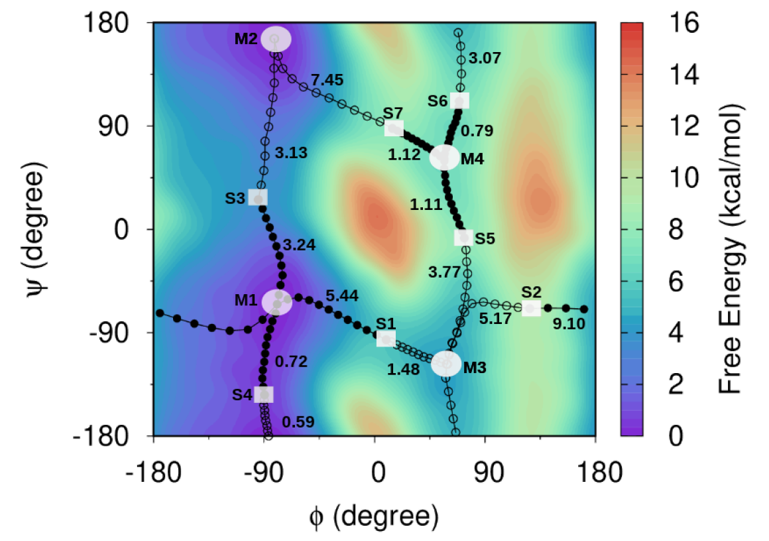
\includegraphics[width=0.85\textwidth]{../ala2network.png}
    };
    \path(g1.north west)
    ++(0,0) node(img1)[anchor=north west]{
        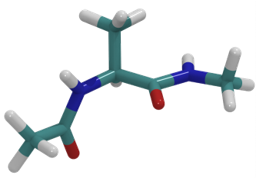
\includegraphics[width=0.25\textwidth]{../ala2m2.png}
    }
    ++(0,0) node(lab1)[anchor=center]{
        {\Large M2}
    };
    \path(g1.south west)
    ++(0,0) node(img2)[anchor=south west]{
        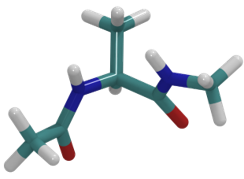
\includegraphics[width=0.25\textwidth]{../ala2m1.png}
    }
    ++(0,0) node(lab1)[anchor=center]{
        {\Large M1}
    };
    \path(g1.south east)
    ++(0,0) node(img3)[anchor=south east]{
        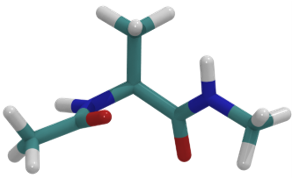
\includegraphics[width=0.25\textwidth]{../ala2m3.png}
    }
    ++(0,0) node(lab1)[anchor=center]{
        {\Large M3}
    };
    \path(g1.north east)
    ++(0,0) node(img3)[anchor=north east]{
        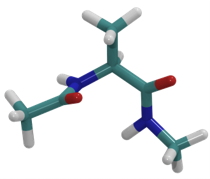
\includegraphics[width=0.25\textwidth]{../ala2m4.png}
    }
    ++(0,0) node(lab1)[anchor=center]{
        {\Large M4}
    };
    \path(se)
    ++(0,0.5) node(att)[anchor=east]{
        {\tiny \textcolor{blue!80!black}{G. Shrivastav and CFA, {\it J Chem Phys} 2019 {\bf 151}:124112}}
    };
\end{tikzpicture}
\end{frame}


\begin{frame}{Climbing Multistrings: Finding Stationary Points, Ala$_3$}
\begin{tikzpicture}
\pcuad{\textwidth}{\textheight}
\path(hl)
    ++(0,-1) node(img1)[anchor=south]{
        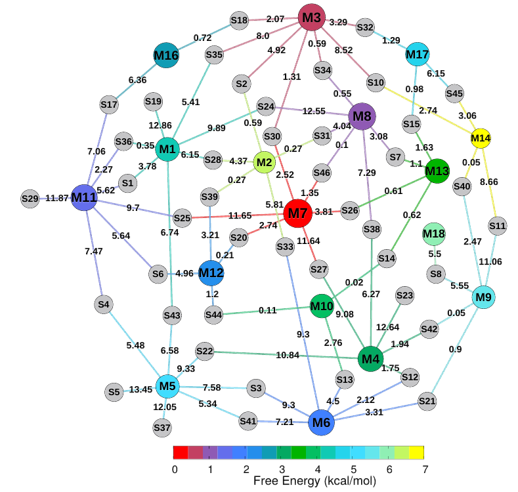
\includegraphics[height=0.6\textheight]{../ala3network.png}
    }
    ++(0.33\textwidth,0.5) node(img2)[anchor=center]{
        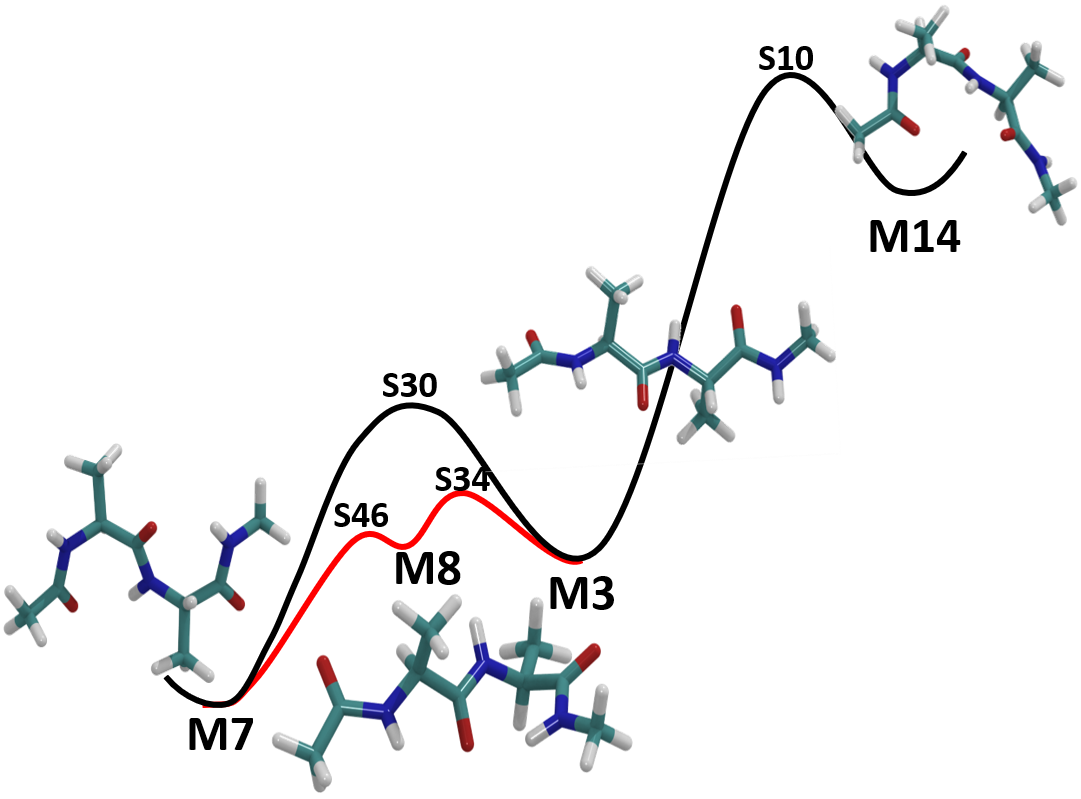
\includegraphics[height=0.7\textheight]{../ala3pathway.png}
    };
\path(se)
    ++(0,0.5) node(att)[anchor=east]{
        {\tiny \textcolor{blue!80!black}{G. Shrivastav and CFA, {\it J Chem Phys} 2019 {\bf 151}:124112}}
    };
\end{tikzpicture}
\end{frame}



\section{Summary}

\begin{frame}[fragile]{Summary}
\begin{itemize}
\item \textcolor{red}{OTFP} combines enhanced sampling and free-energy-profile generation to provide deeper understanding of biomolecular mechanisms
\begin{itemize}
\item We rationalized DAVEI activity dependence on linker length
\item We recapitulate water-mediated ``knock-on'' transport of multiple K$^+$ ions in Kv1.2, but also predict reduced barriers for dry transport
\end{itemize}
\item Demonstrated the \textcolor{magenta!80!black}{Climbing Multistrings Method} for locating stationary points in feature space
\end{itemize}
\end{frame}

\begin{frame}[fragile]{Acknowledgments}
\begin{tikzpicture}[scaleall=1.0]
\pcuad{\textwidth}{\textheight}
%\showcuad
\path(nw) ++(-0.5,0.0) node(text1) [anchor=north west,text width=1.1\textwidth,execute at begin node=\setlength{\baselineskip}{1em}]{
\begin{itemize}
\item {\bf OTFP:}  \textcolor{red!80!black}{Dr. S. Alexis PAZ} (N. U. C\'ordoba, Argentina) and Dr. Steven GOSSERT (2021)
\item {\bf Climbing Multistrings:} \textcolor{green!80!black}{Dr. Gourav SHRIVASTAV}
%\item {\bf Milestoning:} {\small \textcolor{blue!80!black}{Dr. Anthony BUCCI} (West Pharma)}
\item {\bf Other current projects:}
\begin{itemize}
\item Natasha VERGARA (2022):  HIV-1 Entry Inhibitor Design
\item Ming HUANG (2022):  Molecular modeling of thermosets
\item Dr. Salman ZARRINI:  Molecular modeling of thermoset/glass sizing fluid
\item Dr. Ketan KHARE:  Molecular modeling of thermosets
\item Dr. Mohammadjavad MOHAMMADI:  HIV-1 Entry Inhibitor Design
\end{itemize}
\item {\bf Collaborators}
\begin{itemize}
\item \textcolor{magenta!80!black}{Prof. Eric VANDEN-EIJNDEN} (NYU; Mathematics)
\item Prof. Irwin CHAIKEN (DUCOM; Biochemistry)
\item Prof. Amos SMITH III (UPenn; Organic Chemistry)
\end{itemize}
\end{itemize}
\begin{itemize}
\item {\bf Funding (this talk):} {\small NIH R01GM100472, NIH R01GM115249, NSF DMR1207389}
\item {\bf Resources:} {\tt www.github.com/cameronabrams/cfacv}, {\tt www.github.com/cameronabrams/psfgen}, {\tt www.github.com/cameronabrams/otfp}
\end{itemize}
};
\end{tikzpicture}
\end{frame}
  

\end{document}
